\documentclass[utf8, diplomski]{fer}
\usepackage{booktabs}
\usepackage{longtable}
\usepackage{ltablex}
\usepackage{pdfpages}
\usepackage{mathtools}
\usepackage{listings}
\usepackage{subfig}
\setcitestyle{numbers,square}
\usepackage[export]{adjustbox}
\usepackage{float}
\usepackage{tabularx}
\usepackage{enumitem}
\usepackage{mathrsfs}
\usepackage{multirow}
\usepackage[croatian, onelanguage]{algorithm2e}
\usepackage[a-2u]{pdfx}

\begin{document}
\title{Obrana dubokih konvolucijskih modela od neprijateljskih primjera}
\author{Matej Dobrovodski}
\thesisnumber{2231}

\maketitle
\includepdf[pages=-]{izvornik.pdf}
\zahvala{}
\tableofcontents

\chapter{Uvod}
\section{Raspoznavanje objekata}
Raspoznavanje objekata jedan je od ključnih problema područja računalnog vida. Pri rješavanju problema raspoznavanja objekata se na ulaz nekog sustava dovede slika nekog objekta, a na izlazu se očekuje ispravna klasifikacija u neki od predodređenih razreda. Čovjeku ovaj zadatak ne predstavlja veliki problem, no još uvijek ne postoji zadovoljavajuće rješenje problema koje bi vrijedilo za opći slučaj. Trenutno najbolja takva rješenja temelje se na konvolucijskim neuronskim mrežama. \par
Razvoj konvolucijskih mreža počeo je osamdesetih godina prošlog stoljeća pojavom \textit{neocognitron}-a -- neuronske mreže inspirirane biološkim stanicama vidne kore mozga. Krajem devedesetih godina se pojavljuje konvolucijska neuronska mreža LeNet5. LeNet5 mreža je vrlo uspješno raspoznavala rukom pisane znamenke te je ova mreža bila početna točka za daljnja istraživanja drugih neuronskih mreža. \par
ImageNet projekt je velika baza podataka predviđena za istraživanje područja raspoznavanja objekata \citep{ILSVRC15}. S više od $14$ milijuna slika podijeljenih u $20000$ kategorija, ImageNet skup je daleko najveći slobodno dostupni skup slika. Počevši od 2010. godine, ImageNet projekt organizira godišnje natjecanje, \textit{ImageNet Large Scale Visual Recognition Challenge} (ILSVRC). Veliki skok u točnosti pri raspoznavanju dogodio se 2012. godine kada je konvolucijska neuronska mreža \textit{AlexNet} postigla top-5 pogrešku od samo $15.3\%$, što je bilo $10.8\%$ manje od sljedeće mreže \citep{alexnet}. To je postignuto korištenjem grafičkih procesora pri treniranju, što je potaknulo svojevrsnu revoluciju u području dubokog učenja. \par
Do 2017. godine, većina timova u natjecanju je imala top-5 točnost veću od $95\%$. Danas se u raznim bibliotekama mogu naći unaprijed istrenirane mreže koje postižu vrlo dobre rezultate, primjerice ResNet, Xception i VGG. Sve spomenute mreže postižu vrlo zadovoljavajuće točnosti pri ispitivanju -- top-5 točnosti za ImageNet su iznad $90\%$. No u nastavku rada će biti pokazan oblik napada na konvolucijske modele koji dovodi u pitanje pretpostavku da današnje konvolucijske mreže dobro generaliziraju.
\section{Neprijateljski primjeri}
Krajem $2013.$ godine pojavljuje se prvi izravni ``napad'' na duboke neuronske mreže, gdje je jedna od meta bila prethodno spomenuta uspješna mreža \textit{AlexNet} \citep{Szegedy2014IntriguingPO}. Polazna pretpostavka je da duboki modeli, usprkos tome što dobro generaliziraju, imaju ugrađene svojevrsne \textit{slijepe pjege} koje se isplati istražiti.
\par
Vrijedi da za neki ispravno klasificirani ulaz $\boldsymbol{x}$ postoji područje $\boldsymbol{x} + \boldsymbol{r}$ u blizini ulaza te je uobičajeno da modeli ulazne vrijednosti iz tog područja također ispravno klasificiraju, isto kao i $\boldsymbol{x}$. U općem slučaju vrijedi da neprimjetne perturbacije iz tog područja (npr. nasumični šum slabog intenziteta) ne mijenjaju izlaz modela. To je pretpostavka lokalne generalizacije i tipično vrijedi za probleme iz područja računalnog vida.
\par
Međutim, ispostavilo se da pretpostavka lokalne generalizacije ne vrijedi uvijek. Moguće je konstruirati perturbaciju $\boldsymbol{r}$ koja dovodi do pogrešne klasifikacije slike $\boldsymbol{x} + \boldsymbol{r}$, a ljudskom oku nije uočljiva. Takve slike se nazivaju neprijateljskim primjerima, a taj pojam se može generalizirati i na mnoga druga područja i na sličan način se mogu napasti sustavi pretvaranja teksta u govor, sustavi za detekciju zloćudnih programa i praktički svi sustavi koji se oslanjaju na dosadašnje modele dubokog učenja. 
\par
Ono što je iznenađujuće i što je potaklo daljnje istraživanje je to što je zapravo iznimno lako za pronaći takve neprijateljske primjere na \textit{state of the art} modelima kod kojih je perturbacija $\boldsymbol{r}$ potpuno neprimjetna i to što nije nimalo očito zašto mreže neispravno klasificiraju takve ulaze. Jedan od originalnih napada je prikazan na slici \ref{fig:alexnet_adv} gdje ranije spomenuta AlexNet mreža predviđa da su novonastale slike zapravo slike noja.

\begin{figure}[H]
\centering
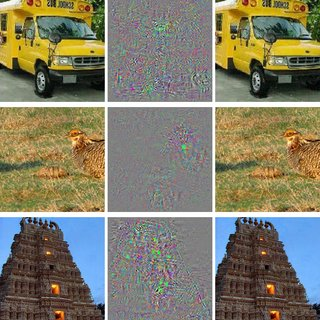
\includegraphics[width=0.5\textwidth,keepaspectratio]{img/other/alexnet_adv.jpg}
\caption{Primjer suparničkog napada na AlexNet mrežu \citep{Szegedy2014IntriguingPO}. U lijevom stupcu su originalne, ispravno klasificirane slike. U srednjem stupcu se nalazi perturbacija koja se nadodaje na originalnu sliku, a u desnom stupcu su sve tri novonastale slike klasificirane kao noj.}
\label{fig:alexnet_adv}
\end{figure}

\par
Motivacija za istraživanje neprijateljskih primjera je višestruka. Jedan od razloga je zaštita postojećih dubokih modela od zlonamjernih neprijateljskih napada. Uz to, vrlo bitan razlog je i produbljivanje postojećeg teorijskog znanja o dubokim modelima. Pojava neprijateljskih primjera nije izolirana niti rijetka, a jednostavnost kojom se konstruiraju je svakako zanimljiva. Dapače, u zadnjih nekoliko godina je područje neprijateljskih primjera doživjelo svojevrsnu eksploziju. U trenutku pisanja ovog rada je približno jednak broj radova na temu neprijateljskih primjera objavljeno u prethodnoj godini dana kao i svih godina prije toga. Ovo se vidi i na slici \ref{fig:cumsum_adv} koja prikazuje graf ukupnog broja radova na temu neprijateljskih primjera počevši od $2014.$ godine.

\begin{figure}[H]
\centering
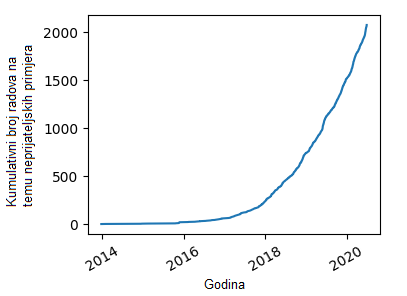
\includegraphics[width=0.8\textwidth,keepaspectratio]{img/other/cumsum.png}
\caption{Ukupan broj radova na temu neprijateljskih primjera kroz godine \citep{carlini_webpage}.}
\label{fig:cumsum_adv}
\end{figure}

U radu je dan pregled nekoliko metoda generiranja neprijateljskih primjera. Neke metode su prikazane zbog njihove povijesne važnosti i utjecaja na daljnji razvoj metoda, dok su neke metode iznimno snažne i mjerilo uspješnosti obrane od suparničkih napada. Pokazano je i koliko su postojeći napadi uspješni protiv poznatih mreža te kako niti jedan od korištenih modela nije unaprijed otporan na napade. Uz napade su pokazane i neke obrane, s naglaskom na njihovu (ne)uspješnost pri odupiranju od postojećih suparničkih napada, probleme koji su gotovo svim obranama zajednički te potencijalnu budućnost razvoja uspješnijih obrana.


\chapter{Programska potpora}
\section{Odabir biblioteke za duboko učenje}
Postoji mnogo biblioteka koje pružaju sve potrebno za duboko učenje i računalni vid. U nastavku rada se koristi \textit{Tensorflow} 2 \citep{abadi2016tensorflow} u kombinaciji s bibliotekom \textit{Keras} \citep{chollet2015keras}. Zbog ogromnog dobitka u brzini izvođenja, ove biblioteke su korištene zajedno s platformom \textit{CUDA} koja omogućava iskorištavanje grafičkog procesora za obradu opće namjene (engl. \textit{graphics processing unit for general purpose processing}, GPGPU). Grafička kartica korištena u sklopu generiranja rezultata u radu je NVIDIA GeForce RTX 2060 SUPER.
\section{Biblioteke za neprijateljske primjere}
Usprkos tome što su suparnički primjeri relativno nov koncept, već postoji mnogo biblioteka koje pružaju implementaciju velikog broja suparničkih napada, a često su i napadi implementirani izravno od strane autora napada. Istaknule su se tri biblioteke za generiranje suparničkih napada: \textit{CleverHans} \citep{papernot2018cleverhans}, \textit{Foolbox Native} \citep{rauber2017foolbox} i \textit{Adversarial Robustness Toolbox (ART)} \citep{art2018}.
\par
Za odabir biblioteke je razmatrano nekoliko stvari: dostupnost i ekstenzivnost dokumentacije, raznovrsnost implementiranih napada, jednostavnost korištenja, zahtijevana programska potpora te postoji li implementacija obrana. Za svaku biblioteku je implementirano generiranje neprijateljskih primjera napadom FGSM koji je opisan u potpoglavlju \ref{fgm}, a napad je proveden na model opisan u potpoglavlju \ref{custom_model}.
\par
\textit{Cleverhans} ima kratku dokumentaciju za sve napade i poveznicu na relevantni rad koji opisuje napad, međutim ne postoji dokumentacija u formatu koji se lako pretražuje. \textit{Foolbox} i \textit{ART} imaju dokumentaciju dostupnu u takvom formatu, međutim \textit{Foolbox} dokumentacija ne opisuje kako se napad poziva i s kojim argumentima, što otežava korištenje bez detaljnijeg proučavanja izvornog kôda, dok je \textit{ART} dokumentacija eksplicitna kod toga.
\par
Što se tiče jednostavnosti korištenja, \textit{Cleverhans} je bio najjednostavniji za primjenu u ovom jednostavnom primjeru. \textit{Foolbox} zahtijeva da se slike pretvore u određen format prije pokretanja napada, što otežava korištenje. \textit{ART}, međutim, zahtijeva dodatne informacije pri konstruiranju napada kao što su broj razreda, dimenzije ulaza, funkcija gubitka i granične vrijednosti, što druge biblioteke ne traže. K tome je vrijeme izvođenja bilo najbrže za \textit{ART}. Ovo je bitno jer se korišteni napad često koristi pri evaluaciji određenih obrana.
\par
\textit{Cleverhans} i \textit{Foolbox} imaju vrlo specifične zahtjeve za programsku potporu, iako će \textit{Cleverhans} u budućnosti podupirati više od samo \textit{Tensorflow}. \textit{ART} pruža potporu za mnoštvo biblioteka: \textit{Tensorflow} (v1 i v2), \textit{Keras}, \textit{PyTorch}, \textit{MXNet} i još neke.
\par
Od navedenih biblioteka, \textit{ART} je jedina koja već sada ima implementirane neke od obrana u literaturi. \textit{Cleverhans} biblioteka ima planove za implementaciju obrana u budućnosti, dok \textit{Foolbox} podržava samo napade.
\par
Zbog svega navedenog, u nastavku rada se koristi \textit{Adversarial Robustness Toolbox}. Dodatno, autori biblioteke su vrlo aktivni na \textit{GitHub}-u i iznimno brzo reagiraju kada se postavi pitanje ili prijavi problem. Pri izradi rada otkriveno je nekoliko \textit{bug}-ova koji su popravljeni u najkraćem roku.

\section{Skupovi podataka}
ImageNet je široko korištena baza podataka slika s preko $14$ milijuna slika raspoređenih u više od $20000$ razreda \citep{ILSVRC15}. ImageNet je praktički postao standard za treniranje i evaluaciju rada modela pri klasifikaciji objekata. Neki od modela korišteni u radu su unaprijed trenirani na ImageNet bazi podataka na kojima postižu iznimno visoku točnost.
\par
Neke obrane i posljedično napadi će u nastavku rada biti evaluirani na CIFAR-10 skupu podataka \citep{cifar10}. CIFAR-10 sadrži samo $10$ disjunktnih razreda, te $50000$ slika za treniranje mreže. Nužno je koristiti i ovaj skup podataka jer pojedine obrane još uvijek nije moguće skalirati na ImageNet razinu jer vrijeme izvođenja nije razumno.
\par
U svrhu rada je također odabrano $16$ slika koje bi ImageNet modeli trebali ispravno klasificirati. Popis slika i izlazi određenih modela nalaze se u privitku\textsuperscript{\ref{dodatak}}.
\section{Konvolucijski modeli}\label{custom_model}
Primarna meta napada u radu je mreža ResNet V2 \citep{resnetv2}, i to verzija s 50 slojeva koja je unaprijed trenirana na ImageNet skupu. Mreža postiže top-1 točnost od $76\%$, te top-5 točnost od $93\%$.  U početnim fazama izrade rada razmatrano je više mreža, međutim ResNet mreža je puno brža pri evaluaciji što ubrzava i olakšava evaluaciju napada i obrana. Korištenje ove mreže ne smanjuje općenitost ideja predstavljenih u radu, pošto su sve konvolucijske mreže jednako ranjive na neprijateljske napade. Lakoća provođenja neprijateljskih napada je ``problem'' koji sve konvolucijske mreže dijele u jednakoj mjeri, i trenutno ne postoji niti jedna takva mreža koja je sama po sebi otporna na njih. Dodatno, kôd priložen uz rad podupire provođenje napada na sljedeće mreže: DenseNet121, VGG16, VGG19, MobileNetV2 te Xception.
\par
Osim ResNet mreže, dodatno je konstruirana i jednostavna konvolucijska mreža za klasifikaciju CIFAR-10 slika. Mreža se sastoji od 11 slojeva, redom:
\begin{enumerate}[noitemsep, label=\textbullet]
  \item konvolucijski sloj oblika $32\times32\times32$ s filtrom veličine $3\times3$
  \item konvolucijski sloj oblika $32\times32\times32$ s filtrom veličine $3\times3$
  \item sloj sažimanja oblika $2\times2$
  \item sloj ispadanja s vjerojatnošću $0.25$
  \item konvolucijski sloj oblika $16\times162\times64$ s filtrom veličine $3\times3$
  \item konvolucijski sloj oblika $16\times162\times64$ s filtrom veličine $3\times3$
  \item sloj sažimanja oblika $2\times2$
  \item sloj ispadanja s vjerojatnošću $0.25$
  \item potpuno povezani sloj veličine $512$
  \item sloj ispadanja s vjerojatnošću $0.50$
  \item potpuno povezani sloj veličine $10$, pošto se klasificira u 10 razreda
\end{enumerate}

\begin{figure}[H]
\centering
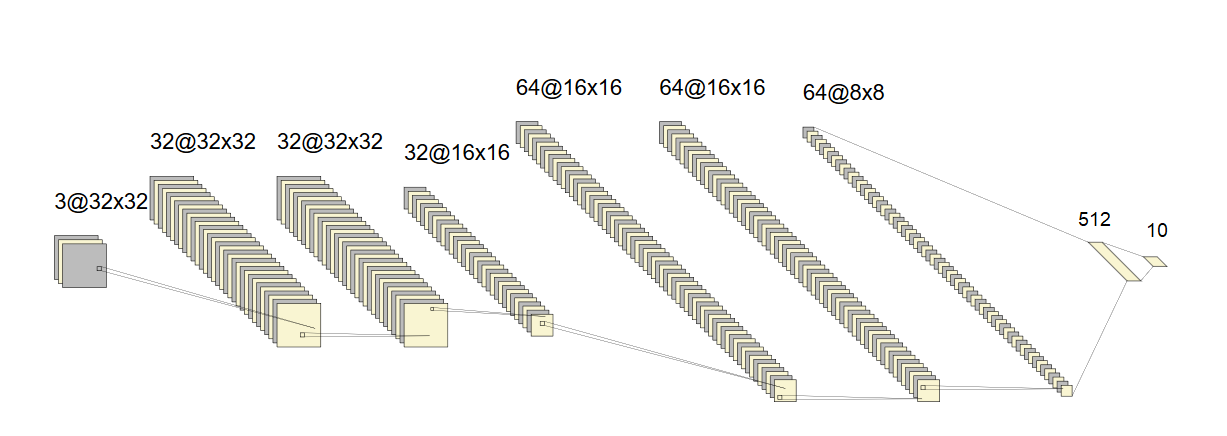
\includegraphics[width=1\textwidth,keepaspectratio]{img/other/toy_cifar10.png}
\caption{Skica jednostavne mreže za CIFAR-10 mrežu. Nisu prikazani slojevi ispadanja.}
\label{fig:toy_cifar10}
\end{figure}

Ukupno mreža ima $2,168,362$ parametara koji se mogu naučiti. Na slici \ref{fig:toy_cifar10} je skica mreže. Aktivacijska funkcija između relevantnih slojeva je \textit{ReLU}. Mreža već nakon $15$ epoha lako postiže točnost od $75\%$ na skupu za testiranje korištenjem optimizacijskog algoritma Adam \citep{adam} uz pretpostavljene zadane hiperparametre od strane \textit{Tensorflow} biblioteke. Nakon $25$ epoha postiže točnost od $79.47\%$, no i u tom trenutku mreža nije pretrenirana. Za potrebe rada nije nužno maksimizirati točnost jer ne bi bitno utjecalo na rezultate. Jednako je lagano za pronaći suparničke primjere i na vrlo dobro istreniranim dubokim mrežama kao i na ovakvim jednostavnim mrežama.


\chapter{Neprijateljski primjeri I}
\section{Model prijetnje}
Model prijetnje (engl. \textit{threat model}) je proces kojim se potencijalne prijetnje mogu nabrojati i identificirati te se mogu odrediti određene mjere kao prioritet. Neki od dijelova modela prijetnje mogu biti: frekvencija interakcije s metom napada, željena vrsta pogrešne klasifikacije, količina znanja o meti napada i specifičnost napada. Prije opisivanja navedenih aspekata modela prijetnje uvedeno je nekoliko relevantnih simbola koji se učestalo pojavljuju u literaturi i u ovom radu.

\begin{table}[H]
\textbf{Osnovni pojmovi i simboli} \\
\begin{tabular}{ l c l }
\textbullet \ $f(\cdot)$ & -- & model dubokog učenja \\ 
\textbullet \ $\boldsymbol{x}$, $l$ & -- & originalni ulaz te pripadajuća labela \\  
\textbullet \ $\boldsymbol{x}'$, $l'$ & -- & neprijateljski primjer i pripadajuća labela \\
\textbullet \ $J(\cdot)$ & -- & funkcija gubitka, u većini slučajeva gubitak unakrsne entropije \\
\textbullet \ $||\cdot||_{p}$ & -- & p-norma, p je najčešće $0$, $2$ ili $\infty$. Dodatna oznaka za norme je $\ell_{p}$.
\end{tabular}
\end{table}

\begin{table}[H]
\textbf{Norme} \\
\begin{tabular}{ l c p{13cm} }
\textbullet \ $\ell_{0}$ & -- & $||\boldsymbol{x}||_{0}$ predstavlja broj ne-nula elemenata vektora $\boldsymbol{x}$.\\ 
\textbullet \ $\ell_{2}$ & -- & $||\boldsymbol{x}||_{2} := \sqrt{x_{1}^{2} + ... + x_{n}^{2}}$, odnosno Euklidska norma.\\
\textbullet \ $\ell_{\infty}$ & -- & $||\boldsymbol{x}||_{\infty} := \max\limits_{i} |x_{i}|$. U kontekstu neprijateljskih napada ova norma predstavlja maksimalnu vrijednost perturbacije $r$. 
\end{tabular}
\end{table}


\begin{table}[H]
\textbf{Frekvencija interakcije s metom napada}
\begin{tabularx}{\textwidth}{ l c X }
\textbullet \ Jednokratni napad & -- & jednokratni napadi (engl. \textit{one-time}) su napadi kojima je potreban samo jedan pristup modelu da generiraju neprijateljski primjer. Ovi napadi su brzi, ali i mnogo slabiji od iterativnih napada te nisu u fokusu istraživanja. Na primjer, napad opisan u potpoglavlju \ref{fgm} je jednokratni napad. \\ 
\textbullet \ Iterativni napad & -- & iterativni napadi zahtijevaju više pristupa modelu da bi generirali neprijateljski primjer. Ovakvi napadi generiraju daleko bolje neprijateljske primjere. Većina napada pripada ovoj kategoriji.
\end{tabularx}
\end{table}

\begin{table}[H]
\textbf{Vrsta pogrešne klasifikacije}
\begin{tabularx}{\textwidth}{ l c X }
\textbullet \ Lažno pozitivni napad & -- & lažno pozitivni (engl. \textit{false positive}) primjeri u kontekstu neprijateljskih napada kod klasifikacijskih problema su čovjeku potpuno neprepoznatljivi (npr. šum), dok mreža s visokom vjerojatnošću klasificira sliku. \\ 
\textbullet \ Lažno negativni napad & -- & lažno negativni (engl. \textit{false negative}) primjeri su oni koje čovjek vrlo lako prepozna, a mreža pogrešno klasificira zbog nevidljive perturbacije. Fokus rada su od početka lažno negativni primjeri. Usporedba napada dana je u slici \ref{fig:fp_fn}.
\end{tabularx}
\end{table}


\begin{figure}[H]
  \centering
  \subfloat[Lažno pozitivni napad. Mreža klasificira sliku kao prostirka za molitvu (engl. \textit{prayer rug}) s vjerojatnošću $98.66\%$.]{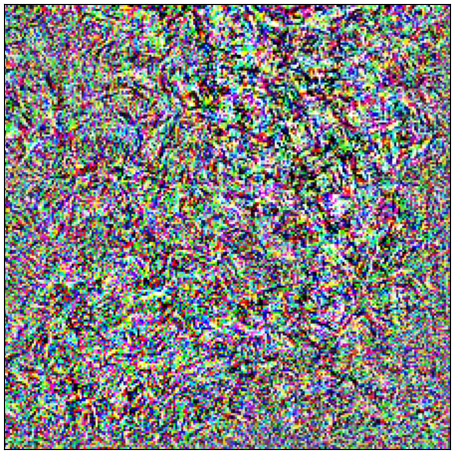
\includegraphics[width=0.48\textwidth]{img/results/prayer_rug_98-66_resnet_cw.png}\label{fig:a}}
  \hfill
  \subfloat[Lažno negativni napad. Mreža klasificira sliku kao zmaj (engl. \textit{kite}) s vjerojatnošću $91.89\%$.]{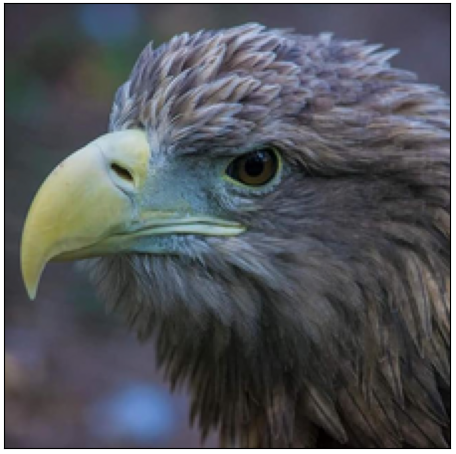
\includegraphics[width=0.48\textwidth]{img/results/kite_91-89_resnet_cw.png}\label{fig:b}}
  \caption{Primjeri lažno pozitivnog i lažno negativnog napada. Napad proveden na ResNet50V2 mreži korištenjem $\ell_{2}$ napada Carlijina i Wagnera opisanog u potpoglavlju \ref{cw}.}
\end{figure}\label{fig:fp_fn}


\begin{table}[H]
\textbf{Znanje o meti napada}
\begin{tabularx}{\textwidth}{ l c X }
\textbullet \ Bijela kutija & -- & model se naziva bijela kutija (engl. \textit{white box}) ako je sve o modelu unaprijed poznato napadaču, uključujući: arhitekturu, parametre mreže, aktivacijske funkcije, hiperparametre i sve druge moguće detalje mreže. Napadi koji se temelje na modelu bijele kutije često iskorištavaju gradijente mreže pri konstruiranju neprijateljskog primjera. \\ 
\textbullet \ Crna kutija & -- & suprotno tome, model crne kutije (engl. \textit{black box}) pretpostavlja nedostatak svih mogućih informacija, osim izlaza iz mreže. Na primjer, ako se napada neka mreža ``u oblaku'', njoj se pristupa tako da joj se preda ulaz te nije moguće direktno saznati dodatne detalje o mreži. Začudo, moguće je konstruirati neprijateljske primjere samo na temelju izlaza mreže.
\end{tabularx}
\end{table}

\begin{table}[H]
\textbf{Specifičnost napada}
\begin{tabularx}{\textwidth}{ l c X }
\textbullet \ Ciljani napad & -- & ciljani napad (engl. \textit{targeted attack}) je oblik napada gdje se za neki neprijateljski primjer pokušava dobiti unaprijed određen izlaz mreže. Uz to, dodatni zahtjev može biti i da se maksimizira vjerojatnost odabranog razreda. \\ 
\textbullet \ Neciljani napad & -- & neciljani napad (engl. \textit{untargeted attack}) zahtijeva jedino da je klasifikacija neprijateljskog primjera neispravna. Općenito je lakše i brže konstruirati neciljani napad.
\end{tabularx}
\end{table}

\section{Pojava prvih neprijateljskih primjera}
U uvodu je opisana osnovna ideja neprijateljskih primjera iz jednog od najranijih radova na temu neprijateljskih primjera \citep{Szegedy2014IntriguingPO}, a u nastavku je ideja dodatno razrađena i ukratko opisana optimizacijska metoda generiranja suparničkih primjera.
\par
Implicitno je pretpostavljeno da mreže imaju svojstvo lokalne generalizacije. Za neki dovoljno mali radijus $\epsilon > 0$ u blizini ulaza $\boldsymbol{x}$ (epsilon okolina), postoji ulaz $\boldsymbol{x} + \boldsymbol{r}$ takav da je $||\boldsymbol{r}|| < \epsilon$ koji će također imati veliku vjerojatnost pripadanja ispravnom klasifikacijskom razredu na izlazu mreže. Slabo vidljive promjene u pravilu ne mijenjaju drastično izlaz mreže, što se može i pokazati dodavanjem šuma na neku ulaznu sliku. Dapače, neke mreže su nasumičnom deformacijom ulaza pri treniranju povećavale robusnost modela. Pokazalo se da svojstvo lokalne generalizacije zapravo u velikoj mjeri nije prisutno kod današnjih modela dubokog učenja i da je moguće osmisliti optimizacijski proces koji će pronaći primjere sa slabo vidljivim promjenama koje ipak drastično mijenjaju izlaz mreže i prisile model na pogrešnu klasifikaciju. Dodatno, spomenuti oblik treniranja deformiranjem ulaza nije nimalo osporavao traženje neprijateljskih primjera.
\par
Slijedi formalni opis optimizacijskog problema koji je potrebno riješiti. \\
Klasifikator koji na ulazu prima sliku, a na izlazu daje pripadnu labelu označen je s $f : \mathbb{R}^{m} \rightarrow \{1...k\}$. Pripadajuća funkcija gubitka definirana je s $loss_{f} : \mathbb{R}^{m}\times\{1...k\} \rightarrow \mathbb{R}^{+}$. Za neku sliku $\boldsymbol{x} \in \mathbb{R}^{m}$ i neku labelu $l \in \{1...k\}$, potrebno je riješiti sljedeći optimizacijski problem:
\begin{enumerate}[noitemsep, label=\textbullet]\label{original_formulation}
  \item minimizirati $||\boldsymbol{r}||_{2}$ uz ograničenja
  \begin{enumerate}
  \item $f(\boldsymbol{x}+\boldsymbol{r}) = l$
  \item $\boldsymbol{x} + \boldsymbol{r} \in [0, 1]^{m}$
  \end{enumerate}
\end{enumerate}
Problem postaje netrivijalan kada labela $l$ nije jednaka izlazu za originalni ulaz, odnosno kada je različita od $f(\boldsymbol{x})$. Traženje egzaktnog $\boldsymbol{r}$ je težak problem. Autori su riješili približni problem:
\begin{enumerate}[noitemsep, label=\textbullet]
  \item minimizirati $c||\boldsymbol{r}||_{2} + loss_{f}(\boldsymbol{x} + \boldsymbol{r}, l)$ uz ograničenje $\boldsymbol{x} + \boldsymbol{r} \in [0, 1]^{m}$
\end{enumerate}
Korištenjem iterativnog optimizacijskog algoritma L-BFGS (engl. \textit{Limited memory Broyden–Fletcher–Goldfarb–Shanno algorithm}) u svakoj iteraciji se minimizira $loss_{f}(\boldsymbol{x} + \boldsymbol{r}, l)$ te se dodatno linijskim pretraživanjem odredi i minimalni $c$ za koji je izlaz takav da je klasifikacija pogrešna. Za rad algoritma L-BFGS potrebno je unaprijed poznavati i vrijednost gradijenta funkcije koja se optimizira, što ovaj napad čini napadom bijele kutije. \par
Jedno od ponuđenih objašnjenja postojanja neprijateljskih primjera je to što su konvolucijske mreže vrlo nelinearne po prirodi. To je zapravo poželjno svojstvo dubokih mreža, jer nelinearnost omogućuje rješavanje vrlo nelinearnih optimizacijskih problema kao što je klasifikacija slika. No čini se da je upravo zbog toliko visoke nelinearnosti lako za pronaći neprijateljske primjere koji su se sakrili u ``džepovima'' u blizini nekog ulaza, koje je vrlo teško pronaći nasumičnim pretraživanjem. 
\section{Brza metoda temeljena na gradijentima}\label{fgm}
Iako su neprijateljski primjeri otkriveni već krajem $2013.$, idući bitni rad na temu neprijateljskih primjera pojavio se tek $2015.$ godine \citep{Goodfellow2015ExplainingAH}. Taj rad je direktni nastavak na prethodni te nudi nove načine generiranja neprijateljskih primjera, jedno novo bitno i zanimljivo svojstvo neprijateljskih primjera te neočekivano objašnjenje postojanja neprijateljskih primjera.
\par
Neprijateljski primjeri su se originalno pojavili pod pretpostavkom da su duboki modeli previše nelinearni te je njihovo postojanje objašnjeno teorijom da modeli imaju ``slijepe pjege'' u kojima se neprijateljski primjeri teško pronalaze. \\
Usprkos tome što je prethodno ponuđeno objašnjenje postojanja neprijateljskih primjera vrlo logično, sljedeći napad je osmišljen počevši od potpuno obrnute pretpostavke.
\par
Ispostavilo se da su i linearni modeli podložni neprijateljskim primjerima, stoga je prvo potrebno objasniti kako je to moguće. \\
Digitalne slike uglavnom koriste samo 8 bitova za reprezentaciju pojedinog piksela, i svaka dodatna informacija manja od $1/255$ je odbačena. Razumno je za očekivati da klasifikator nema različit izlaz za $\boldsymbol{x}$ i $\boldsymbol{\tilde{x}} = \boldsymbol{x} + \boldsymbol{r}$, ako je svaki element perturbacije $\boldsymbol{r}$ manji od spomenute preciznosti. Formalnije, klasifikator bi trebao dati isti izlaz za $\boldsymbol{x}$ i $\boldsymbol{\tilde{x}}$ dokle god je $||\boldsymbol{r}||_{\infty} < \epsilon$, gdje je $\epsilon$ dovoljno malen da bude odbačen. \\
Skalarni umnožak vektora težina $\boldsymbol{w}^{T}$ i primjera s perturbacijom $\boldsymbol{\tilde{x}}$ može se raspisati ovako:
\begin{equation}
	\boldsymbol{w}^{T}\boldsymbol{\tilde{x}} = \boldsymbol{w}^{T}\boldsymbol{x} + \boldsymbol{w}^{T}\boldsymbol{r}
\end{equation}
Dakle, perturbacija $\boldsymbol{r}$ uzrokuje porast aktivacije za $\boldsymbol{w}^{T}\boldsymbol{r}$. Ovaj porast se može maksimizirati postavljanjem $\boldsymbol{r} = \epsilon \text{ sign}(\boldsymbol{w})$. Ako je prosječna vrijednost vektora težina označena s $m$ i broj elemenata vektora je $n$, onda je porast iznosa $\epsilon mn$. Norma $||\boldsymbol{r}||_{\infty}$ ne raste s porastom dimenzionalnosti problema, dok porast aktivacije raste linearno s $n$. Dakle, za visoko dimenzionalne probleme moguće je dodati nevidljive promjene koje onda zajedno mogu drastično promijeniti izlaz.
\par
Ideja je zato napasti klasifikator ``gdje najviše boli''. Potrebno je maksimizirati promjenu izlaza uz minimalnu promjenu svakog pojedinačnog elementa. Za nelinearne modele, ideja je identična: \\
ako su $\boldsymbol{\theta}$ parametri modela, $\boldsymbol{x}$ ulaz, $y$ izlaz te $J(\boldsymbol{\theta}, \boldsymbol{x}, y)$ funkcija gubitka korištena za treniranje mreže, maksimalna perturbacija za koju je uvjet norme zadovoljen je:
\begin{equation}
	\boldsymbol{r} = \epsilon \text{ sign}(\nabla_{x}J(\boldsymbol{\theta}, \boldsymbol{x}, y))
\end{equation}
Ova metoda generiranja neprijateljskih primjera se zove metoda temeljena na predznaku gradijenta (engl. \textit{fast gradient sign method}, FGSM). Metoda je brza jer je potreban samo jedan pristup mreži, i također je napad na bijelu kutiju.
Činjenica da je nelinearne klasifikatore moguće napasti s istom pretpostavkom kao i linearne, te da su nelinearni modeli jednako podložni neprijateljskim napadima kao i linearni modeli dodatno dokazuje da problem nije to što su duboki modeli previše nelinearni, nego to da su previše linearni. Na sličan način se može dobiti maksimalna perturbacija pod uvjetima normi $\ell_{1}$ i $\ell_{2}$. Ne uzme se funkcija predznaka $\text{sign}$ nego je potrebno gradijent podijeliti s određenim faktorom koji osigurava da uvjet norme ostane zadovoljen. Ovako proširena skupina neprijateljskih napada se zove brza metoda temeljena na gradijentima (engl. \textit{fast gradient method}). \\
\begin{figure}[H]
\centering
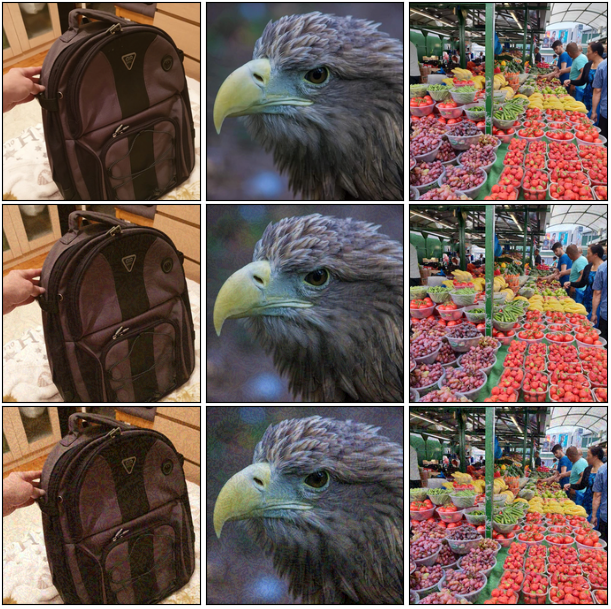
\includegraphics[width=0.9\textwidth,keepaspectratio]{img/results/fgm_inf_1510.png}
\caption{FGSM napad za $\epsilon \in \{1, 5, 10\}$. Torba je predviđena kao nogometna lopta ($99.87\%$, $71.24\%$, $48.63\%)$, orao kao zmaj ($99.76\%$, $99.96\%$, $98.98\%$), i tržnica kao banana ($99.79\%$, $99.99\%$, $99.99\%$).}
\end{figure}\label{fgsm_ex}
Na slici \ref{fgsm_ex} se nalazi primjer FGSM napada. Već za $\epsilon > 2$ FGSM uspješno nalazi neprijateljski primjer za $14/16$ slika iz skupa podataka \ref{osobni_skup}. FGSM ne nađe neprijateljski primjer za slike \ref{ref_pi01} i \ref{ref_pi12} za razumni $\epsilon$. Dodatno je zanimljivo kako kad mreža pogriješi, greška je s vrlo visokom vjerojatnošću. \\
Ranije spomenuto bitno svojstvo neprijateljskih primjera je to da neprijateljski primjeri generaliziraju između različitih modela. Primjer prenosivosti je dan u pododjeljku \ref{transferability} gdje se konstruirani neprijateljski napadi na jednom modelu iskoriste za napad na drugi model.
\section{DeepFool}
Algoritmi FGM uspješno nalaze neprijateljske primjere iz jednog pokušaja. Očito je da bi neka iterativna metoda sigurno pronašla neprijateljske primjere s još manjim perturbacijama.
\par
$2016.$ godine se pojavljuje sljedeći bitan algoritam stvaranja neprijateljskih primjera: DeepFool.\\
DeepFool je iterativni algoritam baziran na modelu bijele kutije. Kao i FGM, DeepFool iskorištava pretpostavljeno svojstvo prevelike linearnosti modela te u svakom koraku aproksimira nelinearni klasifikator na linearan način. Slijedi opis rada DeepFool algoritma na binarnom klasifikatoru. \\
Za neki klasifikator $f$, izlazna labela za neki ulaz $\boldsymbol{x}$ označena je s $\hat{k}(\boldsymbol{x})$. Minimalna perturbacija $\boldsymbol{r}$ je ona koja je dovoljna da promijeni vrijednost izlaza klasifikatora:
\begin{equation}
	\Delta (\boldsymbol{x}; \hat{k}) := \mathop{\min}_{\boldsymbol{r}} ||\boldsymbol{r}||_{2} \text{ uz uvjet } \hat{k}(\boldsymbol{x}+\boldsymbol{r}) \neq \hat{k}(\boldsymbol{x})
\end{equation}
Minimalna perturbacija potrebna za pogrešnu klasifikaciju nekog uzorka se također naziva i robusnost $\hat{k}$ u točki $\boldsymbol{x}$. Usput se može i definirati robusnost cijelog modela:
\begin{equation}
	\rho_{\text{adv}}(\hat{k}) = \mathbb{E}_{\boldsymbol{x}} \frac{\Delta (\boldsymbol{x}; \hat{k})}{||\boldsymbol{x}||_{2}}
\end{equation}
Robusnost nekog klasifikatora definirana je kao očekivana potrebna perturbacija za stvaranje neprijateljskog primjera preko (nekog) cijelog skupa podataka. \\
Za binarni klasifikator $f(\boldsymbol{x})$ se pretpostavlja da vrijedi $\hat{k}(\boldsymbol{x}) = \text{sign}(f(\boldsymbol{x}))$. Dodatno se definira skup $\mathscr{F} := \{\boldsymbol{x} : f(\boldsymbol{x}) = 0\}$ -- skup vektora $\boldsymbol{x}$ za koje je izlaz klasifikatora $0$. \\
Za klasifikator oblika $f(\boldsymbol{x}) = \boldsymbol{w}^{T}\boldsymbol{x} + b$ robusnost u točki $\boldsymbol{x_{0}}$ je jednaka udaljenosti od $\boldsymbol{x_{0}}$ do hiperravnine definirane s $\mathscr{F} = \{\boldsymbol{x} : \boldsymbol{w}^{T}\boldsymbol{x}+b=0\}$. Ovo je prikazano na slici \ref{fig:deepfool_1d}. \\
Prema tome, da bi se klasifikacija promijenila, potrebna je perturbacija koja će točku $\boldsymbol{x} = \boldsymbol{x}_{0} + \boldsymbol{r}$ staviti na drugu stranu hiperravnine. Minimalna takva perturbacija jednaka je ortogonalnoj projekciji $\boldsymbol{x}_{0}$ na ravninu $\mathscr{F}$. Ova projekcija može se izračunati u zatvorenom obliku:
\begin{equation}
	\boldsymbol{r}(\boldsymbol{x_{0}}) := - \frac{f(\boldsymbol{x_{0}})}{||\boldsymbol{w}||_{2}^{2}}\boldsymbol{w}
\end{equation}
U generalnom slučaju za bilo kakav diferencijabilni klasifikator ne može se vrijednost perturbacije izračunati u zatvorenom obliku. Ovdje se ponovno iskorištava svojstvo klasifikatora da su previše linearni, te se u svakoj iteraciji klasifikator $f$ linearizira u točki $\boldsymbol{x_{i}}$. Minimalna perturbacija takvog linearnog klasifikatora u koraku $i$ računa se na sljedeći način:
\begin{equation}
	\mathop{\text{arg min}}_{\boldsymbol{r}_{i}}||\boldsymbol{r}_{i}||_{2} \text{ uz uvjet } f(\boldsymbol{x}_{i}) + \nabla f(\boldsymbol{x}_{i})^{T}\boldsymbol{r}_{i} = 0
\end{equation}
Izraz uvjeta predstavlja tangencijalnu hiperravninu na funkciju klasifikatora u točki $\boldsymbol{x}_{i}$. Algoritam opisan riječima bi glasio ovako: u svakom koraku algoritma se za trenutnu točku napravi linearna aproksimacija klasifikatora, zatim se napravi ortogonalna projekcija trenutne točke na sjecište tangencijalne hiperravnine i $\mathbb{R}^{n}$. Algoritam se ponavlja dokle god klasifikator ne pogriješi, odnosno dokle god točka ne dođe na granicu klasifikatora. Ilustracija iz rada prikazana na slici \ref{fig:deepfool_2d} vizualno opisuje jedan korak algoritma. Zanimljivo je odmah uočiti kako je često i potreban samo jedan korak algoritma. \\
Kako se višerazredni klasifikator može promatrati kao skupina binarnih klasifikatora, algoritam je moguće poopćiti na višerazredne klasifikatore. Poopćenje na višerazredne diferencijabilne klasifikatore može se naći u izvornom radu \citep{MoosaviDezfooli2016DeepFoolAS}. \\

\begin{figure}[H]
  \centering
  \subfloat[Linearni binarni klasifikator. Minimalna perturbacija potrebna za promijeniti izlaz klasifikatora je ortogonalna projekcija na pravac koji dijeli razrede.]{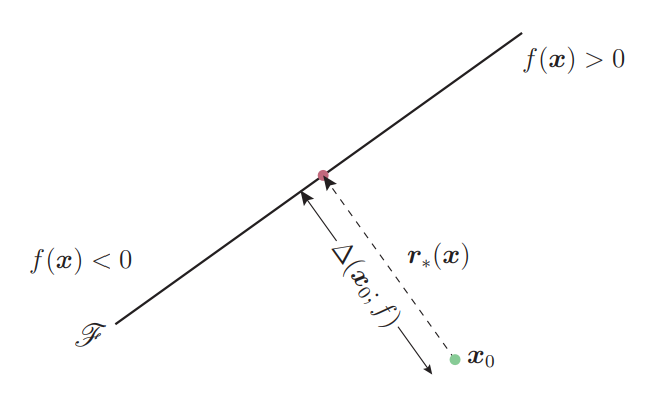
\includegraphics[width=0.49\textwidth]{img/other/deepfool_linear_binary.png}\label{fig:deepfool_1d}}
  \hfill
  \subfloat[Diferencijabilni binarni klasifikator. U svakom koraku se za trenutnu točku aproksimira funkcija klasifikatora s hiperravninom i napravi projekcija na pravac koji je rezultat presjeka dobivene hiperravnine i $\mathbb{R}^{n}$ (označen narančastom bojom).]{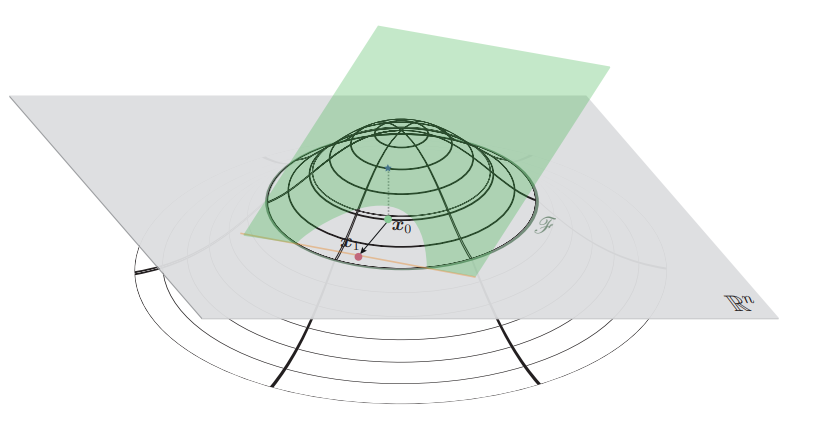
\includegraphics[width=0.49\textwidth]{img/other/deepfool_differential_binary.png}\label{fig:deepfool_2d}}
  \caption{Ilustracija rada DeepFool algoritma na binarnim klasifikatorima \citep{MoosaviDezfooli2016DeepFoolAS}.}
\end{figure}\label{fig:deepfool_illustrations}

Pošto je i za rad ovog algoritma potrebno znanje o mreži, ovo je također napad na model bijele kutije. Za razliku od do sada opisanog FGSM napada, DeepFool pronalazi bolje neprijateljske primjere s daleko manjim perturbacijama. \par
Što se tiče uspješnosti DeepFool napada na skup \ref{osobni_skup}, napad je $100\%$ uspješan na svim slikama. Broj iteracija potreban je također iznenađujuće nizak -- za čak sedam slika je potrebna samo jedna iteracija algoritma. Za FGSM napad su se pokazale najzahtjevnije slike \ref{ref_pi01} i \ref{ref_pi12}. Te dvije slike su u slučaju DeepFoola zahtijevale 6 i 8 iteracija. U slici \ref{deepfool_hard} se nalazi prikaz napada na te slike. 

\begin{figure}[H]
\centering
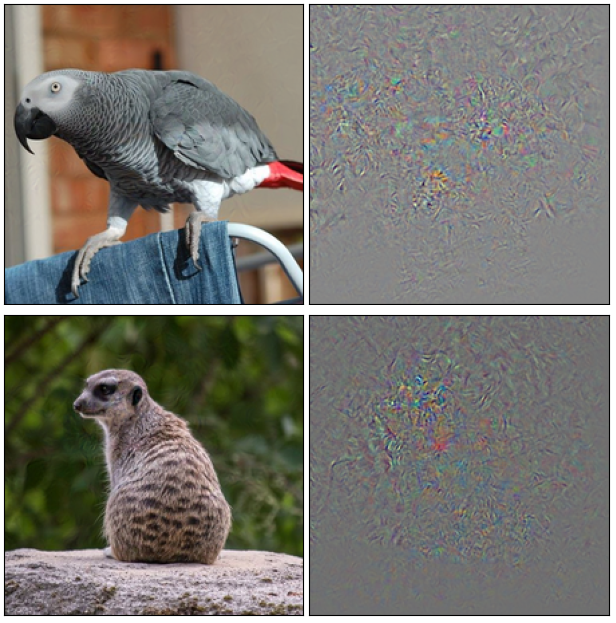
\includegraphics[width=0.9\textwidth,keepaspectratio]{img/results/deepfool_hard.png}
\caption{Rezultati DeepFool napada za slike koje FGSM nije mogao pretvoriti u neprijateljske. U lijevom stupcu je neprijateljska slika, a u desnom je razlika između originalne i neprijateljske slike. Izlaz modela za prvu sliku je \textit{prepelica} (quail, $99.46\%$), a za drugu sliku \textit{šumski kunić} (wood rabbit, $7.8\%$ -- moguće je povećati vjerojatnost uz podešavanje hiperparametara napada)}
\end{figure}\label{deepfool_hard}


\chapter{Obrana dubokih konvolucijskih modela I}
Do sada je predstavljeno nekoliko napada. Originalni napad temeljen na minimizaciji približnog problema uz pomoć L-BFGS algoritam je opisan zbog povijesnih razloga. Napad nije u primjeni jer je u praksi vrlo spor i ne daje dobre rezultate. Međutim, pojavilo se mnoštvo potencijalnih obrana od dosadašnjih napada. U ovom poglavlju su opisane tri glavne kategorije takvih obrana na primjeru pojedinačnih obrana: 
\begin{enumerate}[noitemsep, label=\textbullet]
\item Jednostavne obrane -- konceptualno vrlo jednostavne za shvatiti, nije potrebno duboko predznanje o napadima, ``jeftine'' za implementirati
\item Neprijateljsko treniranje -- osnovna ideja je poboljšanje robusnosti klasifikatora još pri treniranju
\item Prikrivanje gradijenata -- vođeni idejom povećanja nelinearnosti mreže, određene obrane namjerno ili slučajno ``prikrivaju'' gradijente mreže i time prividno sprječavaju napade koji se temelje na gradijentima
\end{enumerate}

\section{Jednostavne obrane}
U ovom dijelu je ukratko opisano nekoliko vrlo jednostavnih obrana. Dobra strana ovih obrana je što su iznimno jednostavne za implementirati i vrlo učinkovite protiv već stvorenih neprijateljskih primjera, te nije potrebno nikakvo mijenjanje samog modela niti detaljno poznavanje potencijalnih metoda napada. Negativno je to što su pre-jednostavne da bi spriječile stvaranje novih neprijateljskih primjera te ne povećavaju robusnost mreže. Općenito, obrane koje su ``agnostičke'' što se tiče modela kojeg brane, odnosno nezavisne su od modela, su u pravilu neuspješne.
\subsection{JPEG kompresija}\label{jpeg_comp}
JPEG kompresija u obliku obrane od neprijateljskih primjera se pojavila više puta u različitim oblicima \citep{jpeg1, jpeg2, jpeg3}, a slijedi opis najjednostavnijeg načina zaštite. \\
JPEG je vrsta sažimanja podataka s gubitkom (engl. \textit{lossy}) za slike. Upravo to svojstvo je poželjno pri uništavanju neprijateljske perturbacije. Pretpostavka je da su i sami neprijateljski primjeri osjetljivi na perturbacije, odnosno da će male promjene nad pažljivo-konstruiranom perturbacijom vratiti sliku nazad u područje ispravne klasifikacije. Ovo dodatno ima smisla kada se uzme u obzir da su neprijateljski primjeri rijetki, to jest da ih nije lako nasumično pronaći. \\
JPEG kompresija bazira se na diskretnoj kosinusnoj transformaciji (engl. \textit{discrete cosine transform}, DCT). Transformacijom iz prostorne domene u frekvencijsku domenu omogućava se direktna manipulacija frekvencijskom domenom. Ljudski vid nije toliko osjetljiv na komponente visoke frekvencije u slikama, stoga se provodi kvantizacija frekvencija te se visoke frekvencije čuvaju s manjom preciznošću nego niske frekvencije. Preciznost pri kojoj se čuvaju visoke frekvencije ovisi o faktoru kvalitete koji je u rasponu od $0$ do $100$: za $0$ se visoke frekvencije potpuno odbacuju, a za $100$ visoke frekvencije su maksimalno očuvane. Važno je uočiti da kvaliteta od $100$ ne znači da je kompresija bez gubitka, jer se gubitak djelomično dogodi već pri prelasku u frekvencijsku domenu. Na slici \ref{fig:jpeg_examples} se nalazi usporedba kompresije za različite kvalitete.

\begin{figure}[H]
\centering
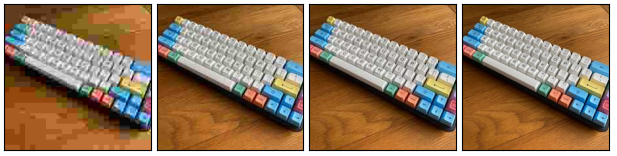
\includegraphics[width=0.9\textwidth,keepaspectratio]{img/other/jpeg_examples.png}
\caption{Primjeri JPEG kompresije za različiti parametar kvalitete. Kvaliteta je redom $5$, $25$, $50$, $90$.}
\label{fig:jpeg_examples}
\end{figure}

\par
Najjednostavnija verzija obrane (i prva koja se pojavila) je korištenje JPEG kompresije samo pri evaluaciji. Autori su isprobali FGSM napad uz $\epsilon \in \{1, 5, 10\}$. Koraci su sljedeći:
\begin{enumerate}[noitemsep, label=\textbullet]
  \item izračunati neprijateljske primjere za navedene $\epsilon$
  \item provesti JPEG kompresiju nad običnim slikama i neprijateljskim primjerima
  \item usporediti izlaz modela za sve navedene skupove
\end{enumerate} 
Dodatno bi bilo zanimljivo vidjeti kako obrana utječe na DeepFool napad, pošto DeepFool generira puno manje perturbacije. Rezultati u tablici \ref{jpeg_defense_table} su dobiveni na 16 slika iz \ref{osobni_skup}. 

\begin{table}[H]
\centering
\begin{tabular}{@{}lcl@{}}
\toprule
Ulaz & Kompresija & Točnost \\ \midrule
\multirow{3}{*}{Standardno} & Bez kompresije & $100.00\%$ \\
							& Kvaliteta $50\%$ & $100.00\%$ \\
							& Kvaliteta $75\%$ & $100.00\%$ \\ \midrule
							
\multirow{3}{*}{FGSM $\epsilon = 1$} & Bez kompresije & $31.25\%$ \\
									 & Kvaliteta $50\%$ & $68.75\%$ \\
									 & Kvaliteta $75\%$ & $43.75\%$ \\ \midrule

\multirow{3}{*}{FGSM $\epsilon = 5$} & Bez kompresije & $18.75\%$ \\
									 & Kvaliteta $50\%$ & $12.50\%$ \\
									 & Kvaliteta $75\%$ & $12.50\%$ \\\midrule
									 
\multirow{3}{*}{FGSM $\epsilon = 10$} & Bez kompresije & $12.50\%$ \\
									 & Kvaliteta $50\%$ & $18.75\%$ \\
									 & Kvaliteta $75\%$ & $12.50\%$ \\\midrule
			
\multirow{3}{*}{DeepFool} & Bez kompresije & $0.00\%$ \\
						  & Kvaliteta $50\%$ & $81.25\%$ \\
						  & Kvaliteta $75\%$ & $64.50\%$ \\ \bottomrule

\end{tabular}
\caption{Utjecaj JPEG kompresije na različite neprijateljske primjere. JPEG kompresija u ovom obliku jedino može pokvariti napade male magnitude, no čak i tada nije uvijek uspješna.}\label{jpeg_defense_table}
\end{table}

Zaključak je dakle da je jednostavna obrana temeljena na JPEG kompresiji daleko od korisnog rješenja, bar za FGSM napad. U slučaju DeepFool napada, obrana je puno uspješnija, međutim i tada ne može dosegnuti $100\%$ točnost kao na čistim ulazima, te čak i napad s iznimno malom perturbacijom može zaobići JPEG kompresiju. Dodatno je problematično to što metoda ne može spriječiti nove napade, samo degradirati postojeće neprijateljske primjere. Dapače, ponovi li se DeepFool napad uz JPEG kompresiju na ulazu, napad je opet uspješan $100\%$ vremena na ovom skupu podataka.
\par
Postoje i sofisticiraniji oblici JPEG kompresije kao metode obrane od neprijateljskih primjera \citep{jpeg2}. Moguće je dodatno mrežu trenirati na slikama različite kvalitete kompresije kako bi mreža mogla uspješno klasificirati i slike lošije kvalitete (koje često imaju artefakte). Ovaj proces autori nazivaju ``cijepljenjem'' mreže. Također je moguće imati onoliko modela koliko i različitih kvaliteta JPEG slika i konstruirati ansambl takvih modela. Međutim, u pravilu su obrane temeljene na ansamblima jake onoliko koliko i najjača komponenta ansambla, a pošto JPEG kompresija nije jaka obrana takav ansambl isto nije vrlo jak pri obrani od neprijateljskih primjera.

\subsection{Stiskanje značajki}
Stiskanje značajki (engl. \textit{feature squeezing}) je općeniti pojam koji se može definirati neovisno o neprijateljskim primjerima. Prostori u kojima se nalaze značajke su često bespotrebno veliki te je ideja smanjiti stupnjeve slobode pojedinih značajki i tako ``istisnuti'' manje bitne značajke \citep{squeezing}. JPEG kompresija se isto može smatrati oblikom stiskanja značajki, no u kontekstu neprijateljskih primjera se termin odnosi na dvije metode: redukcija dubine boje slike i zaglađivanje slike. \par
Dva najčešće korištena formata boje slika za klasifikaciju su RGB (npr. CIFAR-10, ImageNet) i sivi tonovi (engl. \textit{grayscale}, npr. MNIST). Za RGB slike, svaki piksel je reprezentiran s $3 \times 8 = 24$ bita, što daje $2^{24}$ mogućih vrijednosti pojedinog piksela. Međutim, za klasifikaciju slika, nije potrebno imati toliko precizne informacije te ljudi mogu lako prepoznati što se na slici nalazi i s manjom dubinom boje. Smanjenjem broja dostupnih bitova se može pokvariti neprijateljska perturbacija i također u teoriji smanjiti prostor gdje se neprijateljski primjeri mogu nalaziti. Na slici \ref{fig:squeeze_bits} je primjer slike s različitim brojem bitova dostupnim za prikaz boje. Korišten broj bitova u originalnom radu je $4$ i $5$.

\begin{figure}[H]
\centering
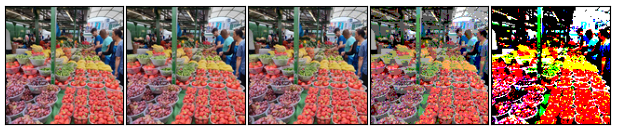
\includegraphics[width=0.9\textwidth,keepaspectratio]{img/other/squeeze_86421.png}
\caption{Ista slika s različitim brojem bitova za boju. Broj bitova je redom $8$, $6$, $4$, $2$ i $1$.}
\label{fig:squeeze_bits}
\end{figure}

Gaussovo zaglađivanje je proces pri kojemu se slika zamućuje do određene mjere. Kao i kod prethodnih metoda, zamućenje može uništiti pažljivo stvorene perturbacije. Na slici \ref{fig:blur_example} se nalazi primjer Gaussovog zamućivanja slike. 

\begin{figure}[H]
\centering
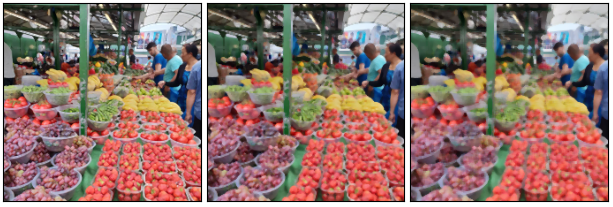
\includegraphics[width=0.9\textwidth,keepaspectratio]{img/other/blur_example.png}
\caption{Zamućenje slike uz veličine prozora $2\times2$, $3\times3$ i $4\times4$}
\label{fig:blur_example}
\end{figure}

\par 

Obje metode su poprilično neuspješne u uništavanju FGSM perturbacije jer je FGSM napad veće magnitude, dok uspješno uništava primjere drugih, jačih napada (npr. DeepFool) koji generiraju manje perturbacije. Ovo je slično kao i kod obrane uz JPEG kompresiju koja je opisana u potpoglavlju \ref{jpeg_comp}. Međutim, kao što se kasnije ispostavilo, obje obrane je vrlo lako zaobići \citep{bypass_squeezing}. Potrebno je jednostavno povećati snagu pojedinih napada da bi se obrane zaobišle, a novonastala perturbacija je također nevidljiva. Postoji i jednostavno objašnjenje zašto Gaussovo zaglađivanje sigurno ne može biti uspješna obrana: zaglađivanje se provodi operacijom konvolucije, što se zapravo može promatrati kao dodatni konvolucijski sloj na ulazu mreže, a konvolucijske mreže su ionako slabe na napade. Stoga još jedan dodatni konvolucijski sloj (s fiksnim težinama) sigurno ne može puno toga napraviti da spriječi nastanak neprijateljskih primjera. Dodatno je zanimljivo i kako se zaglađivanje može koristiti i za generiranje neprijateljskih primjera: dovoljno je linijskim pretraživanjem pronaći najmanji faktor zaglađivanja za koji neka mreža pogriješi. Iznenađujuće je da za puno slika distorzija potrebna za pogrešnu klasifikaciju nije velika. Međutim, ovo se može poboljšati tako da se pri treniranju uvedu i zamućene slike (engl. \textit{data augmentation}).

\section{Neprijateljsko treniranje - FGSM}
Neprijateljsko treniranje se kao ideja pojavila zajedno s FGSM napadom \citep{Goodfellow2015ExplainingAH}. Međutim, neprijateljsko treniranje je tada zamišljeno primarno kao nova metoda regularizacije modela i autori su uspoređivali neprijateljsko treniranje s drugim metodama regularizacije (npr. \textit{dropout} i \textit{pretraining}), a ne kao obranu od potencijalnih neprijateljskih napada. \\
Neprijateljsko treniranje se fundamentalno razlikuje od dosadašnjih metoda povećanja skupa podataka (engl. \textit{data augmentation}). Standardne metode uključuju operacije kao što su rotacija, zrcaljenje, blago mijenjanje boja, brisanje dijelova slike -- no tako transformirane slike i dalje ostaju u originalnoj distribuciji podataka. Zapravo je većina operacija i odabrana upravo iz tog razloga, jer se takve slike očekuju i u skupu podataka za testiranje. No neprijateljsko treniranje trenira model na primjerima koji se nikad ne bi pojavili u skupu za treniranje -- neprijateljski primjeri se ne pojavljuju prirodno nego trebaju biti konstruirani. \par
Najjednostavniji oblik neprijateljskog treniranja je sljedeći:
\begin{enumerate}[noitemsep, label=\textbullet]
  \item u svakom koraku treniranja se skup treniranja podijeli u dva skupa
  \item jedan skup ostane netaknut
  \item drugi skup se pretvori u neprijateljske primjere -- ovo se provodi samo za ulaze koji su ispravno klasificirani
\end{enumerate} 
Omjer skupova je hiperparametar. U originalnom su radu autori odabrali omjer $1:1$ koji radi dovoljno dobro, stoga je i ovdje u nastavku korišten isti omjer.
\par
Za model je ovdje korišten konvolucijski model opisan u potpoglavlju \ref{custom_model}. Model treniran na standardan način nakon $25$ epoha postigne točnost od $78.22\%$, a nakon 50 epoha postigne točnost od $79.80\%$. Za usporedbu, istreniran je model neprijateljskim treniranjem uz FGSM s $\epsilon = 0.1$ te model uz FGSM s $\epsilon \in \{0.05, 0.1, 0.2, 0.3\}$. U slučaju treniranja s više $\epsilon$ vrijednosti se u svakoj iteraciji treniranja uzima iduća $\epsilon$ vrijednost. U tablici \ref{adv_fgsm} se nalaze rezultati uspješnosti FGSM napada uz $\epsilon \in \{0.05, 0.1, 0.2\}$ na različito trenirane modele.

\begin{table}[H]
\centering
\begin{tabular}{@{}lccccc@{}}
\toprule
Treniranje                  & Epoha    & Čisti podatci & {\begin{tabular}[c]{@{}l@{}}FGSM \\ $\epsilon = 0.05$\end{tabular}} & {\begin{tabular}[c]{@{}l@{}}FGSM \\ $\epsilon = 0.1$\end{tabular}} & {\begin{tabular}[c]{@{}l@{}}FGSM \\ $\epsilon = 0.2$\end{tabular}} \\ \midrule
\multirow{2}{*}{Standardno} & $25$ & $78.22\%$ & $19.89\%$ & $16.99\%$ & $16.22\%$ \\
                            & $50$ & $79.80\%$ & $22.05\%$ & $16.85\%$ & $12.32\%$ \\ \midrule
                            
\multirow{2}{*}{\begin{tabular}[c]{@{}l@{}}FGSM $\epsilon = 0.1$\end{tabular}} & $25$ & $73.32\%$ & $44.33\%$ & $66.53\%$ & $23.24\%$ \\
                            & $50$ & $74.96\%$ & $45.89\%$ & $66.14\%$ & $68.33\%$ \\ \midrule
                            
\multirow{2}{*}{\begin{tabular}[c]{@{}l@{}}FGSM $\epsilon = 0.2$\end{tabular}} & $25$ & $74.04\%$ & $15.22\%$ & $24.25\%$ & $69.71\%$ \\
                            & $50$ & $75.77\%$ & $16.80\%$ & $34.47\%$ & $71.11\%$ \\ \midrule
                            
\multirow{2}{*}{\begin{tabular}[c]{@{}l@{}}FGSM $\epsilon = 0.3$\end{tabular}} & $25$ & $74.23\%$ & $15.02\%$ & $18.88\%$ & $56.67\%$ \\
                            & $50$ & $77.76\%$ & $17.12\%$ & $18.30\%$ & $58.76\%$ \\ \midrule
                            
\multirow{2}{*}{\begin{tabular}[c]{@{}l@{}}FGSM $\epsilon\in \{0.05,$ \\ $0.1, 0.2, 0.3\}$\end{tabular}} & $25$ & $77.54\%$ & $43.98\%$ & $73.52\%$ & $30.14\%$ \\
               & $50$ & $76.98\%$ & $66.82\%$ & $69.88\%$ & $69.87\%$\\ \bottomrule
\end{tabular}
\caption{Prikazana je točnost modela na čistim podatcima i uz FGSM za različite $\epsilon$. Neprijateljsko FGSM treniranje ne generalizira preko različitih epsilona, te broj epoha igra bitnu ulogu kod većeg broja napada korištenih pri treniranju.}\label{adv_fgsm}
\end{table}

Neprijateljsko treniranje se čini kao korak u dobrom smjeru, ali ne u ovom obliku. Područje koje je potrebno pokriti je preveliko jer svakako postoji više neprijateljskih primjera nego legitimnih ulaza i jednostavno nije izvodljivo model trenirati na svim normama svakog napada. Bolji oblik neprijateljskog treniranja koji ipak može generalizirati nad različitim normama se dodatno razmatra u potpoglavlju \ref{pgd_adv} s obećavajućim rezultatima.

\section{Termometarsko kodiranje}\label{thermometer}
Termometarsko kodiranje (engl. \textit{thermometer encoding}) je obrana koja je direktno napala problem linearnosti dubokih modela \citep{thermometer_encoding}. Slično kao i prethodne obrane, nije potrebno puno promijeniti postojeći model, ali obrana svejedno nije besplatna kao jednostavnije obrane. \par
Jedan način da se poveća nelinearnost bi bilo mijenjanje aktivacijskih funkcija mreža, no ReLU i ostale aktivacijske funkcije se koriste s razlogom: brze su i jednostavne za optimirati. Druga metoda bi bila da se postavi vrlo nelinearna transformacija na ulaz mreže. Na drugoj metodi se temelji termometarsko kodiranje. \par
Prvo je potrebno uvesti kvantizacijsku funkciju $b$. Potrebno je odabrati vrijednosti $b_{i}$ takve da vrijedi $0 < b_{1} < b_{2} < ... < b_{k} = 1$, npr. $b_{i} = \frac{i}{k}$. Za neki realni broj $\theta \in [0, 1]$ definira se funkcija $b(\theta)$ kao najmanji indeks $\alpha \in \{1, ..., k\}$ takav da je $\theta \leq b_{\alpha}$. \\

Slijedi opis jednojediničnog (engl. \textit{one-hot}) kodiranja. Za neki indeks $j \in \{1, ..., k\}$, neka je $\chi(j) \in \mathbb{R}^{k}$ jednojedinični vektor od $j$:
\begin{equation}
	\chi(j)_{l} = 
	\begin{cases}
      1 & \text{ako } l = j \\
      0 & \text{inače}
    \end{cases}     
\end{equation}
Diskretizacijska funkcija za neki piksel je onda:
\begin{equation}
	f_{\text{onehot}}(x_{i}) = \chi(b(x_{i}))
\end{equation}
Međutim, jednojedinično kodiranje se nije pokazalo dobrom transformacijom ulaza za sprječavanje neprijateljskih primjera. Pretpostavka je da je razlog to što se gubi svojstvo uređenosti između piksela, odnosno za svaku jednojediničnu reprezentaciju vrijedi:
\begin{equation}
	||\chi(b(x_{i}))||_{2} = ||\chi(b(x_{j}))||_{2} = 1 \text{ kada vrijedi } b(x_{i}) \neq b_(x_{j})
\end{equation}
Termometarsko kodiranje je vrlo slično jednojediničnom kodiranju, no ne gubi se svojstvo uređenosti. Za neki indeks $j \in \{1, ..., k\}$, neka je $\tau(j) \in \mathbb{R}^{k}$ termometar vektor od $j$ definiran kao
\begin{equation}
	\tau(j)_{l} = 
	\begin{cases}
      1 & \text{ako } l \geq j \\
      0 & \text{inače}
    \end{cases}     
\end{equation}
Diskretizacijska funkcija za neki piksel je onda:
\begin{equation}
	f_{\text{therm}}(x_{i}) = \tau(b(x_{i}))
\end{equation}
Za svaku termometar reprezentaciju vrijedi:
\begin{equation}
	||\tau(b(x_{i}))||_{2} < ||\tau(b(x_{j}))||_{2} \text{ kada vrijedi } b(x_{i}) \neq b_(x_{j}) \text{ i } x_{i} < x_{j}
\end{equation}

U tablici \ref{example_encoding} je nekoliko primjera jednojediničnog i termometarskog kodiranja.
\begin{table}[H]
\centering
\begin{tabular}{@{}cll@{}}
\toprule
Ulaz & One hot & Termometar\\ \midrule
0.03 & [1000000000] & [1111111111] \\
0.54 & [0000100000] & [0000111111] \\ 
0.78 & [0000000100] & [0000000111] \\ 
0.92 & [0000000001] & [0000000001] \\ \bottomrule
\end{tabular}
\caption{Primjer kodiranja za $b_{i} = \frac{i}{k}$ uz $k = 10$.}\label{example_encoding}
\end{table}
\par
Da bi se neka mreža mogla koristiti s termometarskim kodiranjem, potrebno ju je ponovno istrenirati uz transformaciju ulaza. Nakon $30$ epoha treniranja, mreža na čistim ulazima postiže točnost od $77.13\%$. U ovom obliku, mrežu nije više moguće napasti uspješno niti s jednim od do sada spomenutih napada na model bijele kutije. Razlog tome je što nije moguće obaviti propagaciju unatrag kroz diskretizacijsku funkciju na ulazu i tako dobiti gradijent s obzirom na originalni ulazni podatak (ne-enkodiranu sliku), a većina napada na model bijele kutije koristi tu informaciju. Svi napadi bijele kutije u standardnom formatu imaju uspješnost od približno $0\%$ ako ne uzimaju u obzir transformaciju na ulazu. \\
Autori su zato osmislili dva nova iterativna napada na model bijele kutije koje evaluiraju na istreniranim modelima, te su tako pokazali uspješnost svoje obrane. Ova obrana je bila \textit{state-of-the-art} obrana u trenutku kada se pojavila krajem $2017.$ godine. Međutim, ova i mnoge slične obrane koje pokušavaju diskretizacijom povećati nelinearnost mreže imaju zajednički problem. O tome će biti riječi kasnije u radu.
\pagebreak
\section{Obrambena destilacija}
Obrambena destilacija (engl. \textit{defensive distillation}) je učinkovita obrana koja se temelji na općenitijem pojmu destilacije dubokih neuronskih mreža \citep{Papernot2016DistillationAA}. Destilacija je oblik treniranja mreže koji se provodi u dva koraka. U prvom koraku se standardno trenira neka mreža, no na ulaz u \textit{softmax} sloj se vrijednosti podijele s faktorom $T$ koji se naziva temperatura. Izlaz \textit{softmax} sloja se onda računa prema izrazu u jednadžbi \ref{softmax_t}. Temperatura $T$ igra veliku ulogu u izlazu mreže -- veća temperatura pridaje veću vjerojatnost svim izlazima, i za $T \rightarrow \infty$ vjerojatnost za sve razrede teži k $\frac{1}{K}$. \par

\begin{equation}\label{softmax_t}
	\sigma(\boldsymbol{x})_{i} = \frac{e^{\boldsymbol{x}_{i} / T}}{\sum_{j=1}^{K}e^{\boldsymbol{x}_{j} / T}} \text{ za } i = 1, ..., K \text{ i } \boldsymbol{x} \in \mathbb{R}^{K}
\end{equation}

Nakon treniranja prve mreže, trenira se druga mreža na isti način, ali se u skupu podataka za treniranje labele zamijene izlazom već istrenirane mreže. Stoga se standardne jednojedinične kodirane labele zamjenjuju vjerojatnostima koje je vratila prethodno istrenirana mreža. Ponovno se ponovi postupak treniranja uz temperaturu $T$. Nakon treniranja, za vrijeme testiranja, temperatura $T$ se ukloni, odnosno postavi na $T = 1$. Rezultat je destilirana mreža. \par
U originalnoj formulaciji destilacije mreže, prva mreža je kompleksnija i s većim kapacitetom, dok je druga mreža jednostavnija. Učenje jednostavnije mreže na vjerojatnostima uz temperaturu $T$ se pokazalo korisnim jer jednostavnija mreža uspije postići rezultate neke složenije mreže, a k tome je i brža pri računanju izlaza. \\
U kontekstu obrambene destilacije, obje mreže mogu biti jednake arhitekture. Temperatura je najbitniji parametar, a autori su pokazali da je dobra temperatura $T > 10$. Najbolji rezultati postignuti su za $T = 100$. U tablici \ref{def_destil} su prikazani rezultati različitih FGSM napada te DeepFool napada na destilirane mreže uz temperature $T \in \{50, 100\}$ i rezultati napada na čistu mrežu. Korištena mreža je ponovno CIFAR-10 mreža opisana u potpoglavlju \ref{custom_model}, a treniranje je trajalo $50$ epoha. Mreža trenirana uz $T = 1$ nije destilirana, tu je provedeno standardno treniranje.

\begin{table}[H]
\centering
\begin{tabular}{@{}lccccc@{}}
\toprule
Temperatura & Čisti podatci & {\begin{tabular}[c]{@{}l@{}}FGSM \\ $\epsilon = 2$\end{tabular}} & {\begin{tabular}[c]{@{}l@{}}FGSM \\ $\epsilon = 5$\end{tabular}} & {\begin{tabular}[c]{@{}l@{}}FGSM \\ $\epsilon = 10$\end{tabular}} & DeepFool \\ \midrule
$T = 1$ & $78.89\%$ & $51.47\%$ & $34.87\%$ & $27.99\%$ & $16.80\%$ \\ \midrule
$T = 50$& $78.09\%$ & $77.50\%$ & $77.46\%$ & $76.15\%$ & $77.40\%$ \\ \midrule
$T = 100$ & $78.41\%$ & $78.15\%$ & $78.09\%$ & $77.73\%$ & $76.40\%$ \\ \bottomrule
\end{tabular}
\caption{Točnost za obrambeno destilirane mreže uz različite napade. Mreža za $T = 1$ je trenirana standardno. Napadi imaju iznimno loše rezultate na ovako treniranim mrežama. DeepFool napad je testiran na samo $500$ primjera.}\label{def_destil}
\end{table}
I ova obrana se pokazala iznimno uspješnom na napade na model bijele kutije. Za razliku od termometarskog kodiranja, ovdje je moguće provesti propagaciju unazad, a rezultati su svejedno izvrsni. Nažalost, kao i ranije opisane obrane, i ova obrana ima prikrivenu manu.

\chapter{Neprijateljski primjeri II}
\section{Neučinkovitost obrana}\label{neucinkovitost}
Obrane opisane do sada su se sve pokazale neučinkovitima. Jednostavne transformacije ulaza redovito nisu dovoljne da pokvare perturbacije, a čak i kad jesu, pokazalo se da je moguće konstruirati bolje perturbacije koje su otporne na različite transformacije kao što su JPEG kompresija, zaglađivanje i redukcija dubine boje. Neprijateljsko treniranje uz FGSM ne može generalizirati za različite vrijednosti $\epsilon$, iako je korak u dobrom smjeru. No obrane kao što su termometarsko kodiranje i defenzivna destilacija su se pokazale posebno uspješnima. \par
Maskiranje gradijenata je pojava kod koje model ne sadrži korisne gradijente. Za obrane koje su dizajnirane tako da (namjerno ili slučajno) maskiraju gradijente se kaže da skrivaju gradijente (engl. \textit{gradient obfuscation}) \citep{obfuscated}. Nije svaki oblik maskiranja gradijenata isto što i skrivanje gradijenata -- npr. mreža može naučiti maskirati gradijente, kao što je slučaj kod mnogo oblika neprijateljskog treniranja \citep{ensemble_training}. \par
Oblik skrivanja gradijenata kod obrana koje: nisu diferencijabilne (kao termometarsko kodiranje), su numerički nestabilne, ili na bilo koji način daju neispravne gradijente naziva se \textit{razbijanje gradijenata} (engl. \textit{gradient shattering}) \citep{obfuscated}. U ovu kategoriju spadaju termometarsko kodiranje i defenzivna destilacija. Specifično, termometarsko kodiranje nije diferencijabilno i stoga se ne mogu izravno izračunati gradijenti mreže, što sprječava mnogo napada koji se na tome temelje. \\ Za obrambenu destilaciju je problem malo drukčiji. Temperatura $T$ u \textit{softmax} funkciji efektivno tjera mrežu da izlaze prethodnog sloja skalira za faktor $T$. Kada se pri testiranju opet uzme temperatura $T = 1$, uz velike vrijednosti prethodnog sloja, izlaz mreže postane $\epsilon$ za sve neispravne izlaze, te $1 - N \cdot \epsilon$ za ispravni izlaz. Ispostavilo se da je u većini slučajeva $\epsilon$ toliko malen, da se u 32 bitnoj aritmetici s pomičnim zarezom ta vrijednost zaokruži na $0$ što posljedično i gradijente pretvori u $0$ i tako spriječi napade koji se temelje na gradijentima. \par
Drugi česti problem kod velikog broja ranijih metoda obrane je također to što je njihova evaluacija bila slaba ili nepotpuna. Obrane bi često bile evaluirane na vrlo jednostavnim mrežama, jednostavnim skupovima podataka (CIFAR-10 i MNIST), korištenjem samo najjednostavnijih napada (L-BFGS, FGSM) s nedovoljno dobrim hiperparametrima. Česti problemi evaluacije robusnosti modela su detaljnije opisani u potpoglavlju \ref{preduvjeti}. Kao odgovor na neispravno evaluirane obrane su se pojavili jači napadi koji su korišteni za opovrgavanje uspješnosti tih obrana. U nastavku slijede tri jaka napada: dva na model bijele kutije, te jedan zanimljivi napad na model crne kutije.

\section{Projicirani gradijentni spust}\label{pgd_attack} Projicirani gradijentni spust (engl. \textit{projected gradient descent}) se pojavio u kontekstu neprijateljskog treniranja \citep{Madry2017TowardsDL} koje je detaljno opisano u potpoglavlju \ref{pgd_adv}. Općenito, projicirani gradijentni spust je oblik gradijentnog spusta koji dodatno uzima u obzir ograničenja. Razlika je u tome što je nakon svakog pomaka po gradijentu potrebno obaviti projekciju takvu da su ograničenja zadovoljena. \par 
FGSM napad u jednom koraku izračuna neprijateljski primjer na sljedeći način:
\begin{equation}
	\boldsymbol{\tilde{x}} = \boldsymbol{x} + \epsilon \text{ sign}(\nabla_{\boldsymbol{x}} J(\boldsymbol{\theta}, \boldsymbol{x}, y)) 
\end{equation}
FGSM se može promatrati kao jedan korak iterativnog napada:
\begin{equation}
	\boldsymbol{x}^{t+1} = \Pi_{\boldsymbol{x}+S} (\boldsymbol{x}^{t} + \epsilon \text{ sign}(\nabla_{\boldsymbol{x}} J(\boldsymbol{\theta}, \boldsymbol{x}, y)))
\end{equation}
Operator $\Pi_{\boldsymbol{x}+S}$ predstavlja projekciju na $\boldsymbol{x}+S$. Skup $S \subseteq \mathbb{R}^{d}$ je skup dopuštenih perturbacija. $\boldsymbol{x}+S$ je $\ell_{\infty}$ kugla oko $\boldsymbol{x}$ unutar koje se traže neprijateljski primjeri tako da minimiziraju funkciju $J(\boldsymbol{\theta}, \boldsymbol{x}, y)$. \par

Iako jednostavan, projicirani gradijentni spust je mnogo jači od FGSM i pokazuje svojstva koja ga čine boljim za neprijateljsko treniranje. Već nakon $10$ iteracija uz $\epsilon = 1$ uspješno bude stvoreno $14/16$ neprijateljskih primjera za skup \ref{osobni_skup}. U tablici \ref{pgd_predictions} su predviđanja mreže za tako stvorene primjere. 

\begin{table}[H]
\centering
\begin{tabular}{@{}cll@{}}
\toprule
Slika & Izlaz mreže & Vjerojatnost \\ \midrule
\ref{ref_pi01} & African grey* & $100.00\%$\\
\ref{ref_pi02} & Soccer ball & $100.00\%$ \\ 
\ref{ref_pi03} & Damselfly & $99.94\%$ \\ 
\ref{ref_pi04} & Kite & $99.99\%$ \\  
\ref{ref_pi05} & Banana & $99.99\%$ \\ 
\ref{ref_pi06} & Orangutan & $99.99\%$ \\ 
\ref{ref_pi07} & Pembroke & $98.08\%$ \\ 
\ref{ref_pi08} & Shield & $99.14\%$ \\ 
\ref{ref_pi09} & Dungeness crab & $63.76\%$ \\ 
\ref{ref_pi10} & Space bar & $51.36\%$ \\ 
\ref{ref_pi11} & French bulldog & $99.98\%$ \\ 
\ref{ref_pi12} & Meerkat* & $98.92\%$ \\ 
\ref{ref_pi13} & Welsh springer spaniel & $99.69\%$ \\ 
\ref{ref_pi14} & Neck brace & $100.00\%$ \\ 
\ref{ref_pi15} & Egyptian cat & $99.87\%$ \\ 
\ref{ref_pi16} & Shower curtain & $99.99\%$ \\ \bottomrule
\end{tabular}
\caption{Tablica top-1 izlaza mreže za neprijateljske primjere stvorene PGD algoritmom nakon $10$ iteracija uz $\epsilon = 1$. Slike označene sa zvjezdicom (*) nisu uspješno pretvorene u neprijateljske primjere.}\label{pgd_predictions}
\end{table}

\section{Napadi Carlinija i Wagnera}\label{cw}
Obrambena destilacija naizgled se činila kao vrlo otporna obrana. Problem s gradijentima opisan u potpoglavlju \ref{neucinkovitost} nije inicijalno bio uočen. \\
U svrhu poražavanja obrambene destilacije, autori Carlini i Wagner se vraćaju na početnu definiciju problema neprijateljskih primjera \citep{Carlini2017TowardsET}: 
\begin{enumerate}[noitemsep, label=\textbullet]
  \item minimizirati $\mathcal{D}(\boldsymbol{x}, \boldsymbol{x} + \boldsymbol{r})$ uz ograničenja
  \begin{enumerate}
  \item $C(\boldsymbol{x}+\boldsymbol{r}) = t$
  \item $\boldsymbol{x} + \boldsymbol{r} \in [0, 1]^{m}$
  \end{enumerate}
\end{enumerate}
S $C(\boldsymbol{x})$ je označena labela na izlazu mreže za ulaz $\boldsymbol{x}$. Labela $t$ je proizvoljna, ali problem je netrivijalan samo kad je labela različita od $C(\boldsymbol{x})$. Cilj je dakle pronaći perturbaciju $\boldsymbol{r}$ koja minimizira $\mathcal{D}(\boldsymbol{x}, \boldsymbol{x} + \boldsymbol{r})$. $\mathcal{D}$ je ovdje neka funkcija udaljenosti, na primjer neka od normi $\ell_{1}$, $\ell_{2}$, $\ell_{\infty}$. Potrebno je formulirati problem tako da ga je moguće riješiti nekim od postojećih optimizacijskih algoritama. \\
Definira se funkcija $f$ tako da vrijedi $C(\boldsymbol{x}+\boldsymbol{r}) = t$ ako i samo ako $f(\boldsymbol{x} + \boldsymbol{r}) \leq 0$. Slijedi nekoliko izbora za funkciju $f$:
\begin{enumerate}[topsep=0pt,parsep=0pt,partopsep=0pt, label={}]
	\item $f_{1}(\boldsymbol{x}') = -\text{loss}_{F,t}(\boldsymbol{x}') + 1$
    \item $f_{2}(\boldsymbol{x}') = (\underset{i \neq t}{\max}(F(\boldsymbol{x}')_{i}) - F(\boldsymbol{x}')_{t})^{+}$
    \item $f_{3}(\boldsymbol{x}') = \text{softplus}(\underset{i \neq t}{\max}(F(\boldsymbol{x}')_{i}) - F(\boldsymbol{x}')_{t}) - \log(2)$
    \item $f_{4}(\boldsymbol{x}') = (0.5 - F(\boldsymbol{x}')_{t})^{+}$
    \item $f_{5}(\boldsymbol{x}') = -\log(2F(\boldsymbol{x}')_{t} - 2)$
    \item $f_{6}(\boldsymbol{x}') = (\underset{i \neq t}{\max}(Z(\boldsymbol{x}')_{i}) - Z(\boldsymbol{x}')_{t})^{+}$
    \item $f_{7}(\boldsymbol{x}') = \text{softplus}(\underset{i \neq t}{\max}(Z(\boldsymbol{x}')_{i}) - Z(\boldsymbol{x}')_{t}) - \log(2)$
\end{enumerate}

S $\text{loss}_{F,t}$ je označena funkcija gubitka unakrsne entropije. $(x)^{+}$ označava $\max(x, 0)$, a za $\text{softplus}$ vrijedi $\text{softplus}(x) = \log(1+\exp(x))$. $Z(\boldsymbol{x})$ označava izlaz mreže prije \textit{softmax} sloja -- ove vrijednosti se nazivaju \textit{logiti}. Ovakvom zamjenom je moguće optimizacijski problem formulirati na drugačiji način:

\begin{enumerate}[noitemsep, label={}]
  \item minimizirati $\mathcal{D}(\boldsymbol{x}, \boldsymbol{x} + \boldsymbol{r}) + c\cdot f(\boldsymbol{x} + \boldsymbol{r})$ uz ograničenje $\boldsymbol{x} + \boldsymbol{r} \in [0,1]^{n}$
\end{enumerate}

Još je potrebno razriješiti ograničenje $\boldsymbol{x} + \boldsymbol{r} \in [0,1]^{n}$. U originalnom radu o neprijateljskim primjerima korišten je optimizacijski algoritam L-BFGS koji ovaj oblik ograničenja podržava \citep{Szegedy2014IntriguingPO}. Međutim, moguće je ograničenje riješiti i na drugačiji način: zamjenom varijabli. Umjesto optimizacije varijable $\boldsymbol{r}$, na sljedeći način se uvodi nova varijabla $\boldsymbol{w}$ koju je potrebno optimizirati: 
\begin{equation}
r_{i} = \frac{1}{2}(\tanh(w_{i}) + 1) - x_{i}
\end{equation}
Pošto $-1 \leq \tanh(w_{i}) \leq 1$, i dalje vrijedi $0 \leq x_{i} + r_{i} \leq 1$, pa je rješenje ovog optimizacijskog problema automatski valjano. Ovaj pristup omogućava korištenje optimizacijskih algoritama koji ne podržavaju ograničenja u prethodnom obliku. Autori su odlučili koristiti gradijentni spust uz optimizacijski algoritam Adam. Koeficijent $c$ se traži binarnim pretraživanjem tako da se nađe najmanji $c$ za koji vrijedi $f(\boldsymbol{x}^{*}) \leq 0$ -- za premali $c$, optimizacija ne uspije, a za preveliki $c$ optimizacija uspije, ali napad je manje kvalitete.

Autori provode evaluaciju navedenih $7$ funkcija za različite vrijednosti $c$. Funkcija $f_{6}$ se iskazala kao najuspješnija, stoga je korištena pri formulaciji konačnih napada.

\paragraph{Carlini i Wagner $L_{2}$ napad.} Kombinacijom svega navedenog, dolazi se do konačnog optimizacijskog problema. Za normu je u ovom slučaju uzeta $\ell_{2}$ norma. Napad može biti ciljani, jer se za $t$ može odabrati proizvoljni razred. Optimizacijski problem je onda:

\begin{enumerate}[noitemsep, label=\textbullet]
  \item minimizirati $||\frac{1}{2}(\tanh(\boldsymbol{w}) + 1) - x||_{2}^{2} + c \cdot f(\frac{1}{2}(\tanh(\boldsymbol{w}) + 1))$
\end{enumerate}

gdje je funkcija $f$ definirana na sljedeći način:

\begin{equation}
f(\boldsymbol{x}') = \max(\max\{Z(\boldsymbol{x}')_{i} : i \neq t\} - Z(\boldsymbol{x}')_{t}, -\kappa)
\end{equation}

Parametar $\kappa$ predstavlja ``samouvjerenost'' napada. Za veću vrijednost $\kappa$ pronalazi se neprijateljski primjer za koji će mreža dati veći vjerojatnost. U nastavku se koristi $\kappa = 50$. Na slici \ref{fig:carlini_l2} je prikazan primjer napada na ResNet mrežu.

\begin{figure}[H]
\centering
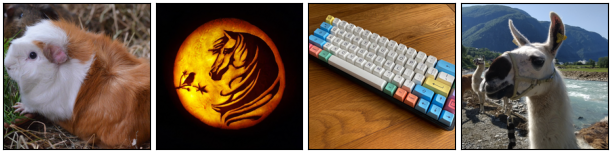
\includegraphics[width=0.95\textwidth,keepaspectratio]{img/results/carlini_l2.png}
\caption{Neciljani CW $\ell_{2}$ napad. Slike su redom klasificirane kao: perzijska mačka, štit, razmak (na tipkovnici) i ovan. Prosječna promjena po pikselu je $0.40$ za ulaz u rasponu $[0, 255]$.}
\label{fig:carlini_l2}
\end{figure}


\paragraph{Carlini i Wagner $L_{\infty}$ napad.} 
$L_{\infty}$ metrika nije u potpunosti diferencijabilna pa gradijentni spust ne radi dobro na naivno postavljenom optimizacijskom problemu:

\begin{enumerate}[noitemsep, label=\textbullet]
  \item minimizirati $c \cdot f(\boldsymbol{x} + \boldsymbol{r}) + ||\boldsymbol{r}||_{\infty}$
\end{enumerate}

Dovoljno je normu zamijeniti s funkcijom koja kažnjava elemente $r_{i}$ koji prelaze vrijednost $\tau$ (inicijalno postavljena na $1$, u svakoj iteraciji se smanjuje za faktor $0.9$):

\begin{enumerate}[noitemsep, label=\textbullet]
  \item minimizirati $c \cdot f(\boldsymbol{x} + \boldsymbol{r}) + \smashoperator[r]{\sum_{i}} [(r_{i} - \tau )^{+}]$
\end{enumerate}

Koeficijent $c$ se ponovno traži binarnim pretraživanjem. Postavi se na neku malu vrijednost i onda se provede optimizacija. Ako ne uspije, $c$ se poveća za faktor $2$ i postupak se ponovi sve dok se ne pronađe dobro rješenje. Na slici \ref{fig:carlini_linf} je prikazan primjer napada na ResNet mrežu.

\begin{figure}[H]
\centering
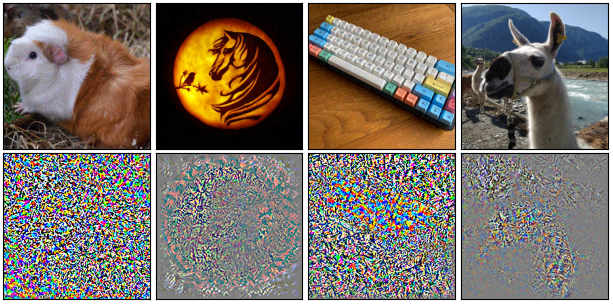
\includegraphics[width=0.95\textwidth,keepaspectratio]{img/results/carlini_linf.png}
\caption{Ciljani CW $\ell_{\infty}$ napad. Sve četiri slike su klasificirane kao sombrero s vjerojatnostima od $92.04\%$, $96.55\%$, $99.73\%$ i $99.85\%$. U donjem redu se nalazi normalizirana razlika između originalne i neprijateljske slike.}
\label{fig:carlini_linf}
\end{figure}

Za $16$ slika u skupu podataka iz \ref{osobni_skup} i ResNet mrežu, $L_{\infty}$ napad je uspješan svaki put za $\epsilon = 6$. $L_{2}$ također uspije svaki put, no za neke teže slike je potrebno dodatno podešavati hiperparametre i rezultat nije idealan za manji broj iteracija. Takve teže slike su \ref{ref_pi01}, \ref{ref_pi03} i \ref{ref_pi12}, a rezultat napada uz pretpostavljene hiperparametre je prikazan na slici \ref{fig:carlini_fail}. Rezultantni neprijateljski primjer za \ref{ref_pi12} i podešene hiperparametre je prikazan na slici \ref{fig:carlini_meerkat}. Prosječna $\ell_{2}$ norma perturbacije na svim primjerima iznosi $8.32$ za ulaz u rasponu $[0, 1]$.

\begin{figure}[H]
\centering
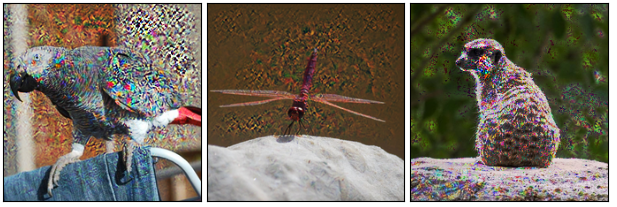
\includegraphics[width=0.9\textwidth,keepaspectratio]{img/results/carlini_fail.png}
\caption{$L_{2}$ napad za teže primjere uz pretpostavljene hiperparametre i mali broj iteracija.}
\label{fig:carlini_fail}
\end{figure}

\begin{figure}[H]
\centering
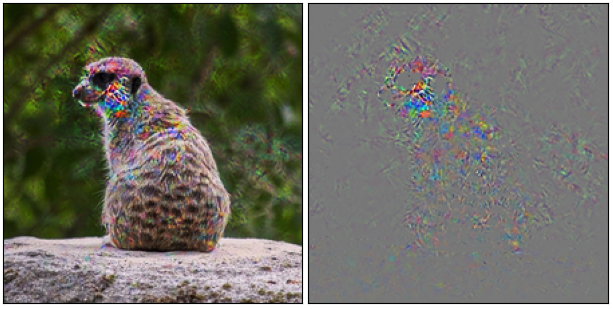
\includegraphics[width=0.9\textwidth,keepaspectratio]{img/results/carlini_meerkat.png}
\caption{Neprijateljski primjer lošije kvalitete uz $L_{2}$ napad. Lijevo je neprijateljska slika klasificirana kao paun (engl. \textit{peacock}) s vjerojatnošću $81.23\%$, a desno je normalizirana razlika naspram originalne slike. $\ell_{2}$ norma perturbacije iznosi $152.39$ za ulaz u rasponu $[0, 1]$.}
\label{fig:carlini_meerkat}
\end{figure}

Problem s obrambenom destilacijom je opisan ranije. Metode napada na model bijele kutije često ovise o gradijentima modela pa su zato i bili neuspješni. Pod ovim napadom, obrambena destilacija pruža minimalnu zaštitu. Rezultati napada su prikazani u tablici \ref{carlini_distillation}.

\begin{table}[H]
\centering
\begin{tabular}{@{}ccc@{}}
\toprule
Čisti podatci & {\begin{tabular}[c]{@{}l@{}}CW $\ell_{\infty}$  \\ $\epsilon = 10$\end{tabular}} & CW $\ell_{2}$\\ \midrule
$78.93\%$ & $9.60\%$ & $10.00\%$ \\ \bottomrule
\end{tabular}
\caption{Rezultati CW napada na obrambenu destilaciju za $T = 100$. Napad $\ell_{\infty}$ je proveden na $500$ primjera, a $\ell_{2}$ na $200$ primjera iz skupa podataka za testiranje.}\label{carlini_distillation}
\end{table}

Ovaj napad se pokazao iznimno uspješnim i teškim za poraziti. Zbog toga je postao standardni napad za evaluaciju obrana. Na slici \ref{fig:mnist_carlini} se nalaze napadi iz originalnog rada na MNIST skup podataka. Arhitektura i način treniranja u izvornom radu nisu pretjerano različiti od opisanog u potpoglavlju \ref{custom_model}.

\begin{figure}[H]
  \centering
  \subfloat[$L_{2}$ napad.]{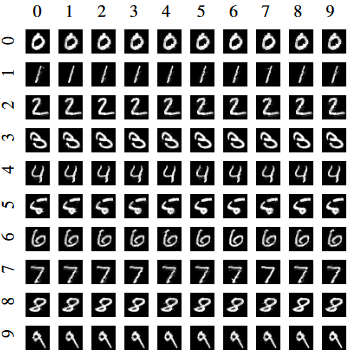
\includegraphics[width=0.48\textwidth]{img/other/carlini_mnist_l2.png}\label{fig:carlini_a}}
  \hfill
  \subfloat[$L_{\infty}$ napad.]{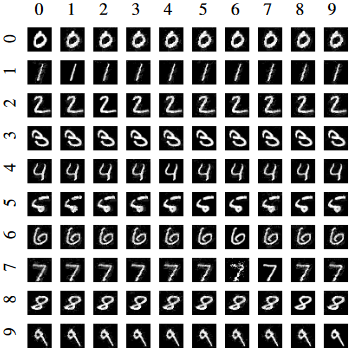
\includegraphics[width=0.48\textwidth]{img/other/carlini_mnist_linf.png}\label{fig:carlini_b}}
  \caption{Primjeri napada na MNIST skup podataka. Na dijagonalama se nalaze izvorne slike. Redovi su ispravne labele, a stupci su izlazne labele nakon ciljanog napada. Slika preuzeta iz \citep{Carlini2017TowardsET}.}
\end{figure}\label{fig:mnist_carlini}

\subsection{Napad na termometarsko kodiranje}

Iako nije izravno vezano uz opisane CW napade, u nastavku je dana ideja napada na termometarsko kodiranje od strane istih autora \citep{obfuscated}. Ova i slične ideje se često primjenjuju pri opovrgavanju obrana koje upotrebljavaju neki nediferencijabilni element. \par
Mnogo nediferencijabilnih obrana se može opisati na sljedeći način: za neki klasifikator $f(\cdot)$ dan je postupak predobrade $g(\cdot)$. Obranjeni klasifikator je onda $\hat{f}(\boldsymbol{x}) = f(g(\boldsymbol{x}))$, a za $g$ vrijedi $g(\boldsymbol{x}) \approx \boldsymbol{x}$. Ovakav $g(\cdot)$ je npr. JPEG kompresija, ali se JPEG kompresija ionako pokazala dovoljno slabom da ju i FGSM može zaobići. \\
S obzirom na to da vrijedi $g(\boldsymbol{x}) \approx \boldsymbol{x}$, derivacija funkcije se može aproksimirati kao derivacija funkcije identiteta, iako je sama transformacija nelinearna. Vrijedi $\nabla_{x}g(\boldsymbol{x}) \approx \nabla_{x} \boldsymbol{x} = 1$. Takve obrane se onda vrlo lako zaobilaze jer se dovoljno dobro mogu procijeniti gradijenti.
\par
Iako je taj pristup efikasan kod obrana gdje stvarno vrijedi $g(\boldsymbol{x}) \approx \boldsymbol{x}$, nije dovoljno generalan za druge nediferencijabilne obrane. Takvo je na primjer termometarsko kodiranje. \\
Neka je neuronska mreža $f(\cdot) = f^{1...j}(\cdot)$, a $f^{i}(\cdot)$ nediferencijabilni sloj. Da bi se aproksimirao $\nabla_{x}f(\boldsymbol{x})$ potrebna je prvo diferencijabilna aproksimacija $g(\boldsymbol{x}) \approx f^{i}(\boldsymbol{x})$. Pri prolazu unazad kroz mrežu se onda $f^{i}(\boldsymbol{x})$ zamijeni s $g(\boldsymbol{x})$. Iako funkcije nisu ekvivalentne, pokazalo se da je ovakva aproksimacija gradijenata dovoljno dobra za konstrukciju neprijateljskih primjera. Ovaj pristup se naziva diferencijalna aproksimacija prolaza unazad (engl. \textit{Backward Pass Differentiable Approximation} -- BPDA).
\par
Termometarsko kodiranje za sliku $\boldsymbol{x}$ je opisano u potpoglavlju \ref{thermometer}. Za piksel $x_{i,j,c}$, termometar enkodirani vektor je zadan s $\tau(x_{i, j, c})_{k} = 1$ ako $x_{i,j,c} > k/l$, a $0$ inače (u ranije opisanom potpoglavlju je nejednadžba bila obrnuta, a posljedično je rezultantni vektor bio negiran, no ovo ne utječe na svojstva obrane). Ako se zada:

\begin{equation}
	\hat{\tau} (x_{i, j, c})_{k} = \min(\max(x_{i,j,c} - k/l, 0), 1)
\end{equation}

onda vrijedi:
\begin{equation}
	\tau (x_{i, j, c})_{k} = \text{floor}(\hat{\tau}(x_{i,j,c})_{k})
\end{equation}

Odabere li se potom $g(\boldsymbol{x}) = \hat{\tau}(\boldsymbol{x})$ moguće je provesti diferencijabilni prolaz unazad kroz mrežu i izračunati približne gradijente. Ovo efektivno poništava obranu i ponovno se mogu koristiti napadi na model bijele kutije kako su prethodno opisani. Pretpostavka da je ova obrana povećala nelinearnost modela je neispravna, obrana se zapravo temeljila na maskiranju gradijenata a takve obrane je redovito lako za poraziti.

\section{Granični napad}\label{boundary_att} Do sada su bili razmatrani samo napadi na model bijele kutije. Takvi napadi su u pravilu jači od napada na model crne kutije jer mogu iskoristiti dodatno znanje o mreže da poboljšaju napad. Napadi na model crne kutije ne znaju ništa o mreži osim vrijednosti izlaza. U praksi, modeli o kojima je znanje minimalno su česti, na primjer modeli kojima se pristupa preko nekakvog web sučelja (npr. \textit{Microsoft Azure} i slični servisi). Usprkos manjku znanja o mreži, moguće je konstruirati vrlo uspješne napade.
Jedan od napada na model crne kutije je granični napad (engl. \textit{boundary attack}) \citep{Brendel2017DecisionBasedAA}. Napad je temeljen na odluci (engl. \textit{decision based attack}), odnosno zahtijeva samo labelu na izlazu mreže. Za razliku od napada temeljenog na odluci, neki napadi crne kutije očekuju i vjerojatnosti na izlazu. \par
Napad započinje iz neke točke koja već je neprijateljska (odnosno pogrešno klasificirana) i iterativno se približava zadanom ulazu $\boldsymbol{x}$ pod uvjetom da je u svakom koraku i dalje neprijateljska. Najjednostavniji opis algoritma je dan u nastavku. Korištena je notacija kao i u izvornom radu \citep{Brendel2017DecisionBasedAA}, stoga je oznaka za ulaz $\boldsymbol{o}$, a oznaka za perturbaciju je $\boldsymbol{\eta}$.

\begin{center}
\begin{algorithm}[H]
 \KwData{ulazna slika $\boldsymbol{o}$}
 \KwResult{neprijateljski primjer $\boldsymbol{\tilde{o}}$ }
 inicijalizacija: $k=0$, $\boldsymbol{\tilde{o}}^{0}$ $\sim \mathcal{U}(0, 1)$ takav da je neprijateljski klasificiran\;
 \While{$k$ < maksimalni broj koraka}{
  odabere se nasumična perturbacija iz distribucije $\boldsymbol{\eta_{k}} \sim \mathcal{P}(\boldsymbol{\tilde{o}}^{k-1})$\;
  \eIf{je $\boldsymbol{\tilde{o}}^{k-1} + \boldsymbol{\eta_{k}}$ neprijateljski}{
   postavi $\boldsymbol{\tilde{o}}^{k} = \boldsymbol{\tilde{o}}^{k-1} + \boldsymbol{\eta_{k}}$\;
   }{
   postavi $\boldsymbol{\tilde{o}}^{k} = \boldsymbol{\tilde{o}}^{k-1}$\;
  }
 $k = k + 1$
 }
 \caption{Najjednostavniji oblik graničnog napada. Potreban je samo izlaz mreže.}\label{simple_boundary_alg}
\end{algorithm}
\end{center}
\par
Ako je napad neciljani, ulazna slika može biti neki šum (pod uvjetom da je šum pogrešno klasificiran). Za ciljani napad, ulazna slika treba biti slika iz ciljanog razreda. Ključni dio algoritma je distribucija $\mathcal{P}$. Optimalna distribucija bi se u pravilu trebala razlikovati između domena problema i različitih modela, no iznenađujuće je kako je moguće uspješno konstruirati neprijateljske primjere uz jednostavnu distribuciju. Perturbacije se generiraju iz distribucije s maksimalnom entropijom uz sljedeća ograničenja:
\begin{enumerate}
  \item Perturbirani uzorak je i dalje u domeni, odnosno:
  \begin{equation}\label{boundary_1_cond}
	\tilde{o}_{i}^{k-1} + \eta_{i}^{k} \in [0, 255]
	\end{equation}
  \item Perturbacija ima relativnu veličinu iznosa $\delta$, odnosno:
    \begin{equation}\label{boundary_2_cond}
	||\boldsymbol{\eta}^{k}||_{2} = \delta \cdot d(\boldsymbol{o}, \boldsymbol{\tilde{o}}^{k-1})\text{, gdje je }d(\boldsymbol{o}, \boldsymbol{\tilde{o}}) = ||\boldsymbol{o} - \boldsymbol{\tilde{o}}||_{2}^{2} \text{ -- udaljenost između }\boldsymbol{o}\text{ i } \boldsymbol{\tilde{o}}
	\end{equation}
	\item Perturbacija smanjuje udaljenost između ciljane slike i perturbirane slike za neki relativni iznos, odnosno:
    \begin{equation}\label{boundary_3_cond}
	d(\boldsymbol{o}, \boldsymbol{\tilde{o}}^{k-1}) - d(\boldsymbol{o}, \boldsymbol{\tilde{o}}^{k-1} + \boldsymbol{\eta}^{k}) = \epsilon \cdot d(\boldsymbol{o}, \boldsymbol{\tilde{o}}^{k-1})
	\end{equation}
\end{enumerate}

Autori su priložili ilustraciju koja slikovito prikazuje rad algoritma. Ilustracija je prikazana na slici \ref{fig:boundary_intuition}.


\begin{figure}[H]
\centering
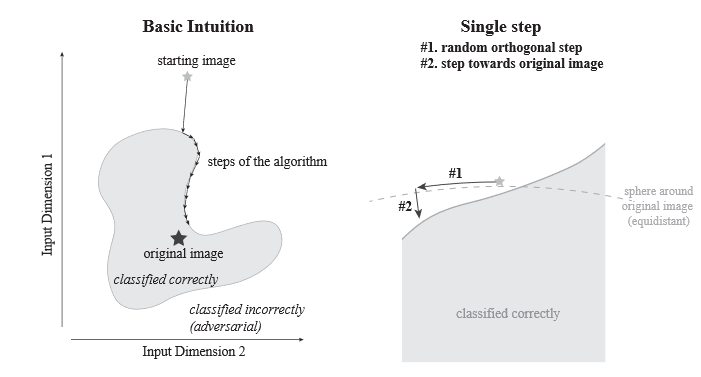
\includegraphics[width=1.0\textwidth,keepaspectratio]{img/other/boundary_intuition.png}
\caption{Na lijevoj slici je prikazan rad algoritma kroz nekoliko koraka. U svakom koraku se neprijateljski primjer približava slici, ali tako da uvijek bude izvan granice ispravne klasifikacije. Na desnoj slici je prikazan jedan korak algoritma. Prvo se napravi nasumičan korak na sferi oko originalne slike, a nakon toga se napravi korak prema originalnoj slici. Slika preuzeta iz \citep{Brendel2017DecisionBasedAA}.}
\label{fig:boundary_intuition}
\end{figure}

Nije lako uzorkovati opisanu distribuciju $\mathcal{P}$, ali je moguće konstruirati jednostavniju heuristiku koja je dovoljno dobra. Prvo se uzorkuje normalna distribucija $\boldsymbol{\eta}_{i}^{k} \sim \mathcal{N}(0, 1)$ nakon čega se uzorak skalira i ograniči tako da zadovoljava ograničenja \ref{boundary_1_cond} i \ref{boundary_2_cond}. U idućem koraku se radi pomak po sferi oko $\boldsymbol{o}$ u nasumičnom smjeru, odnosno mora vrijediti $d(\boldsymbol{o}, \boldsymbol{\tilde{o}}^{k-1} + \boldsymbol{\eta}^{k}) = d(\boldsymbol{o}, \boldsymbol{\tilde{o}}^{k-1})$ i ograničenje \ref{boundary_1_cond}. U zadnjem koraku se pomakne prema originalnoj slici tako da ograničenja \ref{boundary_1_cond} i \ref{boundary_3_cond} budu zadovoljena. Za visoko-dimenzionalne ulaze i dovoljno male $\delta$ i $\epsilon$, ograničenje \ref{boundary_2_cond} će biti praktički zadovoljeno. \par
Postavlja se pitanje što je s lokalnim minimumima. Lokalni minimumi predstavljaju problem utoliko što se na višestruko pokretanje algoritma dogodi konvergencija prema različitim minimumima, ali ti minimumi su sličnog reda veličine. Ne događa se slučaj da algoritam zapne u nekom lokalnom minimumu do te mjere da se ne postigne vizualno prihvatljiv neprijateljski primjer. Ta činjenica ukazuje na ne-robusnost modela. U idealnom slučaju napad se ne bi uspio približiti dovoljno ciljanoj slici da postane kvalitetan neprijateljski primjer. Na slici \ref{fig:boundary_triple} su tri primjera napada. \par

\begin{figure}[H]
\centering
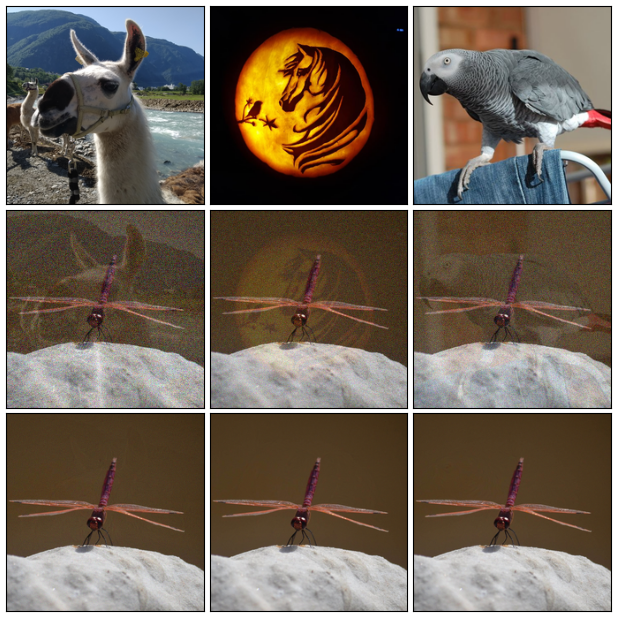
\includegraphics[width=1.0\textwidth,keepaspectratio]{img/results/boundary_triple.png}
\caption{Tri primjera graničnog napada na ResNet mrežu. U prvom redu su originalne slike, u drugom redu je rezultat nakon $400$ koraka, a u trećem redu je rezultat nakon $8000$ koraka. Algoritam jako brzo nađe šumovito rješenje, a onda većinu vremena optimizira neprijateljski primjer, kao što je pokazano na slici \ref{fig:boundary_intuition}. Za svaki pojedini stupac, izlaz modela je isti za svaki red (po stupcima: \textit{llama}, \textit{jack-o'-lantern}, \textit{African grey}).}
\label{fig:boundary_triple}
\end{figure}

Bitno je naglasiti da ni ovako jaki napad ne dolazi besplatno. U usporedbi s napadima bijele kutije, broj evaluacija mreže je veći za nekoliko redova veličine (uz isti cilj, na primjer isti iznos norme). Za DeepFool napad, autorima je u prosjeku trebalo $7$ prolaza kroz mrežu (broj predikcija ulaza) i $37$ prolaza unazad (za računanje gradijenata), dok je za granični napad sličnog iznosa norme potrebno $1,200,000$ prolaza kroz mrežu i $0$ prolaza unazad. Ovo je u slučaju da se žele iznimno dobri rezultati. Na slici \ref{fig:boundary_triple} je napad već nakon $8000$ iteracija postigao vrlo dobar rezultat, a još su k tome i slike birane tako da problem bude teži. Ciljana slika ima vrlo jednostavnu jednobojnu pozadinu i napad je svejedno iznimno uspješan. Jedino se u slučaju ljame vidi obris, no i to bi nestalo nakon mnogo iteracija. Za $8000$ iteracija potrebno vrijeme izvršavanja je preko $8$ sati.

Što se tiče svih prethodno opisanih obrana, za sve postoji napad na model bijele kutije koji ih može poraziti. Slijedi primjer ovog napada na obrane neprijateljskog treniranja (uz FGSM) i obrambenu destilaciju. Napad na obrambenu destilaciju uz $T = 100$ je na slici \ref{fig:boundary_distillation}. Napad na neprijateljski treniranu mrežu uz FGSM je na slici \ref{fig:boundary_fgsm_adv}. \\
Dodatna zanimljivost je to što su autori graničnog napada također autori \textit{FoolBox} biblioteke koja je bila razmatrana za korištenje u sklopu rada.

\begin{figure}[H]
\centering
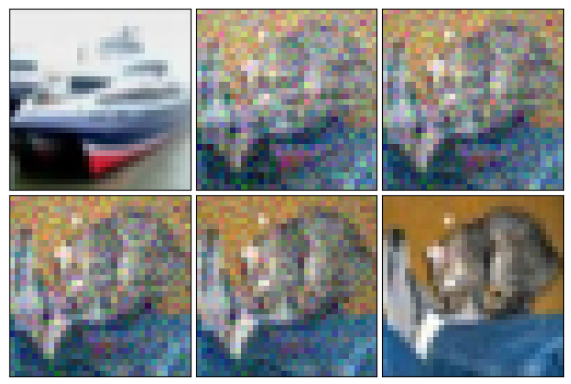
\includegraphics[width=0.9\textwidth,keepaspectratio]{img/results/boundary_distillation.png}
\caption{Napad na obrambenu destilaciju. Slike su nakon svake desete iteracije. Zadnja slika je nakon $2500$ iteracija uz $\ell_{2} = 107.63$ za ulaz u rasponu $[0, 255]$.}
\label{fig:boundary_distillation}
\end{figure}

\begin{figure}[H]
\centering
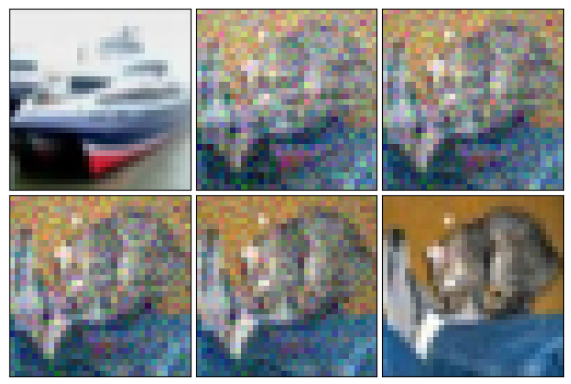
\includegraphics[width=0.9\textwidth,keepaspectratio]{img/results/boundary_distillation.png}
\caption{Napad na neprijateljsko treniranje uz FGSM. Slike su nakon svake desete iteracije. Zadnja slika je nakon $2500$ iteracija uz $\ell_{2} = 101.51$ za ulaz u rasponu $[0, 255]$.}
\label{fig:boundary_fgsm_adv}
\end{figure}

\section{Prenosivost napada}\label{transferability}
Neprijateljski primjeri iskazuju još jedno posebno svojstvo koje je jednako iznenađujuće koliko i zabrinjavajuće. Moguće je konstruirati neprijateljske primjere za neki model, a da ti isti primjeri budu neprijateljski za drugi model. Ovo svojstvo se zove prenosivost (engl. \textit{transferability}) ili generalizacija te je uočeno u isto vrijeme kada je nastao i FGSM napad \citep{Goodfellow2015ExplainingAH}. U nastavku slijede dva primjera: 
\begin{enumerate}[noitemsep, label=\textbullet]
\item Uspješnost prenosivosti napada između dva različita modela
\item Napad na obrambenu destilaciju putem prenosivosti
\end{enumerate}
\subsection{Prenosivost neprijateljskih primjera između modela}\label{model_transferability}
U svrhu provjere svojstva prenosivosti neprijateljskih napada je osmišljen dodatni model. Model se temelji na onom opisanom u \ref{custom_model}, ali je kompleksniji. \\
Mreža se sastoji od 11 slojeva, redom:
\begin{enumerate}[noitemsep, label=\textbullet]
  \item konvolucijski sloj oblika $32\times32\times64$ s filtrom veličine $3\times3$
  \item konvolucijski sloj oblika $32\times32\times64$ s filtrom veličine $3\times3$
  \item konvolucijski sloj oblika $32\times32\times64$ s filtrom veličine $3\times3$
  \item sloj sažimanja oblika $2\times2$
  \item sloj ispadanja s vjerojatnošću $0.2$
  \item konvolucijski sloj oblika $16\times162\times128$ s filtrom veličine $3\times3$
  \item konvolucijski sloj oblika $16\times162\times128$ s filtrom veličine $3\times3$
  \item sloj sažimanja oblika $2\times2$
  \item sloj ispadanja s vjerojatnošću $0.2$
  \item potpuno povezani sloj veličine $1024$
  \item sloj ispadanja s vjerojatnošću $0.50$
  \item potpuno povezani sloj veličine $10$
\end{enumerate}

Broj parametara koje mreža može naučiti je $8,696,970$, a obje mreže su trenirane $50$ epoha uz optimizacijski algoritam Adam. Nakon $50$ epoha, navedena mreža postigne točnost od $81.02\%$. \\
Mreže jesu slične, ali se i u mnogo toga razlikuju. Ponajviše po broju parametara koji se mogu naučiti te nešto drukčijoj arhitekturi. Radi kratkoće i čitkosti, mreža iz \ref{custom_model} je u nastavku označena s $A$, a nova mreža je označena s $B$. Prenosivost je pokazana u oba smjera: koliko su napadi konstruirani pomoću mreže $A$ uspješni na mreži $B$ i koliko su napadi konstruirani pomoću mreže $B$ uspješni protiv mreže $A$. Isprobano je nekoliko verzija FGSM napada te Carlini i Wagner $\ell_{2}$ i $\ell_{\infty}$ napadi. FGSM napad je proveden nad cijelim skupom za testiranje. Carlini i Wagner $\ell_{2}$ napad je proveden samo na prvih $200$ slika, a $\ell_{\infty}$ je proveden na prvih $500$ slika skupa za testiranje. Model $A$ na zadnjih $200$ i $500$ slika postiže točnost od $80.6\%$ i $83.0\%$, a model $B$ postiže točnost od $82.4\%$ i $82.0\%$. Razlog provođenja napada samo na podskupu skupa za testiranje je vrijeme izvođenja. Hiperparametar je $\kappa = 50$ za oba CW napada.

\begin{table}[H]
\centering
\begin{tabular}{@{}cccccc@{}}
\toprule
Model & {\begin{tabular}[c]{@{}l@{}}FGSM \\ $\epsilon = 2$\end{tabular}} & {\begin{tabular}[c]{@{}l@{}}FGSM \\ $\epsilon = 5$\end{tabular}} & {\begin{tabular}[c]{@{}l@{}}FGSM \\ $\epsilon = 10$\end{tabular}} & {\begin{tabular}[c]{@{}l@{}}CW $\ell_{\infty}$  \\ $\epsilon = 10$\end{tabular}} & CW $\ell_{2}$\\ \midrule
$A$ & $51.36\%$ & $32.83\%$ & $22.19\%$ & $38.80\%$ & $10.00\%$\\ \midrule 
$B$ & $79.03\%$ & $72.18\%$ & $54.89\%$ & $49.20\%$ & $46.50\%$\\ \bottomrule
\end{tabular}
\caption{Rezultati neprijateljskih napada generiranih na modelu $A$. Model $A$ je ``jednostavniji''. Napadi s $A$ djelomično prelaze na $B$, a $\ell_{2}$ napad je najučinkovitiji za oba modela.}
\end{table}

\begin{table}[H]
\centering
\begin{tabular}{@{}cccccc@{}}
\toprule
Model & {\begin{tabular}[c]{@{}l@{}}FGSM \\ $\epsilon = 2$\end{tabular}} & {\begin{tabular}[c]{@{}l@{}}FGSM \\ $\epsilon = 5$\end{tabular}} & {\begin{tabular}[c]{@{}l@{}}FGSM \\ $\epsilon = 10$\end{tabular}} & {\begin{tabular}[c]{@{}l@{}}CW $\ell_{\infty}$  \\ $\epsilon = 10$\end{tabular}} & CW $\ell_{2}$\\ \midrule
$A$ & $76.84\%$ & $67.39\%$ & $47.82\%$ & $36.66\%$ & $40.50\%$\\ \midrule 
$B$ & $51.08\%$ & $33.69\%$ & $25.17\%$ & $22.88\%$ & $11.00\%$ \\ \bottomrule
\end{tabular}
\caption{Rezultati neprijateljskih napada generiranih na modelu $B$. Model $B$ je ``kompleksniji''. Napadi konstruirani na $B$ relativno uspješno prelaze na $A$.}
\end{table}

Rezultati su fascinantni. Napadi konstruirani na $A$ modelu prelaze na model $B$ u puno manjoj mjeri nego obrnuto. Napad CW uz $\ell_{\infty}$ normu je zapravo uspješniji na modelu $B$, a još k tome je i uspješniji nego kada se napad izravno provede na $A$. Bitno je ponovno uočiti dvije stvari: 

\begin{enumerate}[noitemsep,topsep=0pt,parsep=0pt,partopsep=0pt, label=\textbullet]
	\item Model $B$ ima otprilike $4$ puta više parametara od modela $A$ i drukčiju arhitekturu
    \item Ovo nipošto ne može biti slučajnost jer nasumični šum ne prouzročuje ni približno toliki pad u točnosti. Ovo je pokazano u tablici \ref{10eps_test}.
\end{enumerate}

\begin{table}[H]
\centering
\begin{tabular}{@{}ccccc@{}}
\toprule
Model & Čisti podatci & {\begin{tabular}[c]{@{}l@{}}Šum od \\ $\epsilon \in [-10, 10]$\end{tabular}} & {\begin{tabular}[c]{@{}l@{}}Gaussov šum s \\ $\mu = 0$ i $\sigma = 5$\end{tabular}} & {\begin{tabular}[c]{@{}l@{}}Šum od \\ $\epsilon \in \{-10, 10\}$\end{tabular}} \\ \midrule
$A$ & $79.80\%$ & $79.53\%$ & $78.87\%$ & $72.81\%$\\ \midrule 
$B$ & $81.02\%$ & $79.54\%$ & $78.67\%$ & $72.22\%$\\ \bottomrule
\end{tabular}
\caption{Točnost modela na čistom CIFAR-10 skupu i na istom skupu uz nasumični šum u rasponu $\epsilon \in [-10, 10]$, Gaussov šum uz $\sigma = 5$ i šum $\epsilon \in \{-10, 10\}$. U svim slučajevima je šum skaliran i slika omeđena ponovo na $[0, 1]$. Ovo je pretpostavka lokalne generalizacije.}\label{10eps_test}
\end{table}

Teorije koje pokušavaju objasniti prenosivost postoje, ali su izvan dosega ovog rada. Dodatno je zanimljivo kako prenosivost ne ovisi čak ni o skupu podataka na kojem se trenira te je moguće napraviti napade koji prelaze s modela na model čak i kada su trenirani na različitim skupovima podataka \citep{Goodfellow2015ExplainingAH}. Prenosivost je bitna pojava koja se treba uzeti u obzir pri evaluaciji obrana. Zato u idućem potpoglavlju slijedi kratka evaluacija obrambene destilacije korištenjem prenosivosti. Naime, robusna mreža ne bi trebala biti podložna ovakvom obliku napada. Na slici \ref{fig:transferability_b_to_a} su prikazani uspješni neprijateljski primjeri koji su preneseni s $B$ na $A$. U prvom redu su originalne slike, a nadalje su u svakom redu neprijateljski primjeri za napade kako su navedeni ranije.

\begin{figure}[H]
\centering
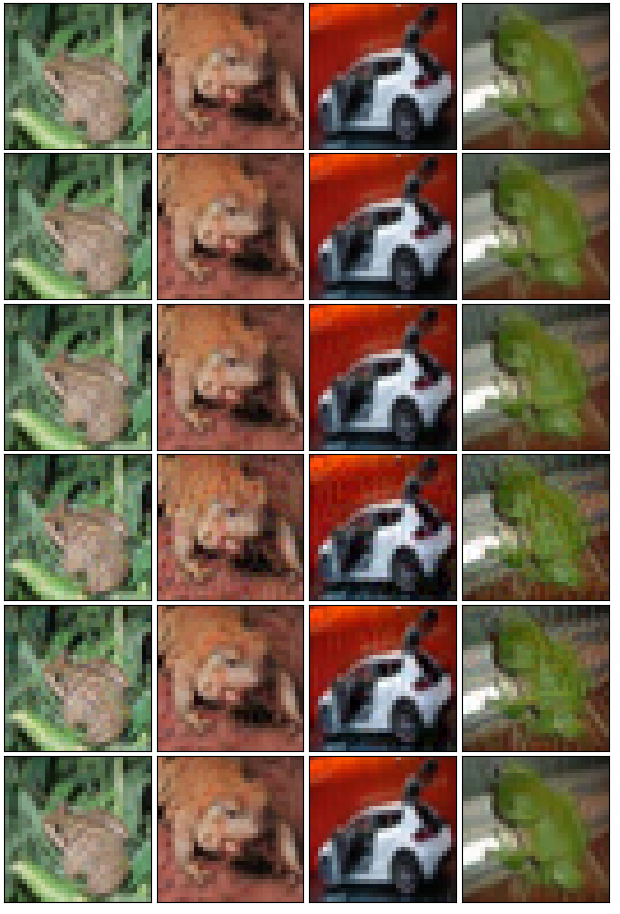
\includegraphics[width=0.85\textwidth,keepaspectratio]{img/results/transferability_b_to_a.png}
\caption{Primjeri uspješno prenesenih neprijateljskih primjera s modela $B$ na model $A$. U prvom redu su originalne slike, iduća tri reda su FGSM napadi te su u zadnja dva reda CW napadi.}
\label{fig:transferability_b_to_a}
\end{figure}


\subsection{Prenosivost neprijateljskih primjera na obrambenu destilaciju}
U \ref{cw} je pokazana uspješnost Carlini i Wagner napada na obrambenu destilaciju. U ovom dijelu je testirana prenosivost FGSM i CW napada na destilirani model. Rezultati se nalaze u tablici \ref{distillation_transfer}. Napad je proveden na standardno treniranom modelu iz \ref{custom_model} nakon $50$ epoha. Hiperparametar je $\kappa = 50$ za oba CW napada, a napad je proveden na $500$ i $200$ slika kao i u prethodnom poglavlju.

\begin{table}[H]
\centering
\begin{tabular}{@{}cccccc@{}}
\toprule
{\begin{tabular}[c]{@{}l@{}}Čisti \\ podatci\end{tabular}} & {\begin{tabular}[c]{@{}l@{}}FGSM \\ $\epsilon = 2$\end{tabular}} & {\begin{tabular}[c]{@{}l@{}}FGSM \\ $\epsilon = 5$\end{tabular}} & {\begin{tabular}[c]{@{}l@{}}FGSM \\ $\epsilon = 10$\end{tabular}} & {\begin{tabular}[c]{@{}l@{}}CW $\ell_{\infty}$  \\ $\epsilon = 10$\end{tabular}} & CW $\ell_{2}$\\ \midrule
$78.41\%$ & $75.39\%$ & $65.47\%$ & $45.65\%$ & $35.20\%$ & $36.00\%$\\ \bottomrule
\end{tabular}
\caption{Prenosivost sa standardno treniranog modela na obrambeno destilirani model.}\label{distillation_transfer}
\end{table}

Zaključak je ponovno da obrambena destilacija ne pruža jaku zaštitu, pogotovo u slučaju CW napada. U potpoglavlju \ref{model_transferability} je provedena evaluacija prenosivosti između dva modela s različitim arhitekturama i brojem parametra. U ovom je slučaju provedena evaluacija prenosivosti između iste arhitekture i jednakog broja parametara, ali s različitim režimom treniranja. 


\chapter{Obrana dubokih konvolucijskih modela II}
\section{Preduvjeti uspješnih obrana}\label{preduvjeti}
Zaključak do sada je da je evaluacija obrana vrlo teška. Usprkos velikom uloženom radu, vrlo malo obrana se uistinu pokazalo uspješnima. Čak i obrane koje su se pokazale uspješnima nisu bile idealno rješenje koje uvijek radi. Jedna od takvih obrana je opisana u potpoglavlju \ref{pgd_adv} i temelji se na ranije opisanom projiciranom gradijentnom spustu. Svakako niti jedna od naizgled idealnih obrana nije dugo opstala, takve su na primjer termometarsko kodiranje i defenzivna destilacija. \par
Potaknuti neuspjehom dosadašnjih obrana, skupina autora prethodno opisanih napada i obrana objavljuju popis principa za uspješnu evaluaciju obrana te česte ``zamke'' s kojima su se prethodne obrane susrele \citep{on_evaluating}. U nastavku su dani neki od bitnih principa i zamki.
\paragraph{Bitni principi pri evaluaciji obrana}
\begin{enumerate}[noitemsep,topsep=0pt,parsep=0pt,partopsep=0pt]
	\item Precizno navesti model prijetnje za koji bi obrana trebala biti uspješna.
    \item Provesti adaptivne napade te dati gornju granicu robusnosti.
    \begin{enumerate}[noitemsep,topsep=0pt,parsep=0pt,partopsep=0pt]
    	\item Adaptivni napadi su napadi koji su izravno prilagođeni obrani. Nije dovoljno isprobati nasumične napade, nego je nužno osmisliti i iskoristiti napad koji se ``prilagodio'' toj specifičnoj obrani.
        \item Napadi moraju imati pristup mreži od početka do kraja.
        \item Fokus treba biti na najjačim takvim napadima.
        \item Potvrditi da adaptivni napadi rade bolje od bilo kojeg drugog oblika napada.
    \end{enumerate}
    \item Podijeliti izvorni kôd obrane i trenirane modele.
    \item Navesti i opisati korištene napade i njihove hiperparametre.
    \item Provjeriti da vrijede najosnovnije i nužne pretpostavke:
    \begin{enumerate}[noitemsep,topsep=0pt,parsep=0pt,partopsep=0pt]
    	\item Provjeriti da iterativni napadi rade bolje od napada od jednog koraka.
        \item Provjeriti da pojačanje perturbacije nužno povećava uspješnost napada.
        \item Provjeriti da se pri velikim perturbacijama model dovodi u stanje ``nasumičnog pogađanja'' izlazne vrijednosti.
    \end{enumerate}
    \item Dati točnost modela bez ikakvog napada.
    \item Evaluirati obranu korištenjem prenosivosti neprijateljskih primjera.
\end{enumerate}


\paragraph{Česte zamke}
\begin{enumerate}[noitemsep,topsep=0pt,parsep=0pt,partopsep=0pt]
	\item Potrebno je obranu evaluirati na širokom skupu napada, posebno u slučaju kada se obranu neprijateljski trenira na samo jednom napadu.
	\item Isprobati barem jedan napad koji ne koristi gradijente te jedan napad koji koristi samo labele.
	\begin{enumerate}[noitemsep,topsep=0pt,parsep=0pt,partopsep=0pt]
    	\item Provjeriti da su napadi koji ne koriste gradijente manje uspješni od napada koji koriste gradijente (inače je velika vjerojatnost da je došlo do maskiranja gradijenata).
    	\item Pažljivo istražiti hiperparametre napada koji utječu na uspješnost.
    \end{enumerate}
    \item Za ne-diferencijabilne komponente, primijeniti diferencijabilne tehnike.
    \item Provjeriti da je napad konvergirao za određene hiperparametre.
    \item Pažljivo odabrati hiperparametre korištenih napada, navesti korištene parametre i opisati njihov utjecaj.
    \item Provjeriti da su iterativni napadi striktno bolji od jednokratnih napada.
    \item Provjeriti da povećanje iznosa dozvoljene perturbacije striktno povećava uspješnost napada.
\end{enumerate}
\medskip
\par
Ovo su samo neki od principa koje bi trebalo slijediti i zamki koje bi trebalo izbjegavati. U stvarnosti je lista mnogo dulja, te svaki pojedini pristup ima svoje posebne napomene, principe i zamke. Ovakve liste se ne bi trebale slijepo pratiti te je uvijek potrebno pristupiti evaluaciji bilo kakvog napada ili obrane na vrlo (samo)kritičan način. Ako se neki bitni principi zanemaruju, bitno je naglasiti i objasniti zašto. 
\par
Postavlja se pitanje zašto je toliki fokus na napade na model bijele kutije i zašto se neka obrana smatra slabom samo zato što ju se može zaobići s vrlo specifičnim napadom. Zapravo se koncept neprijateljskih primjera lako može usporediti s napadom na kriptografski sustav. Kriptografski sustav se ne može smatrati sigurnim samo zato što je crna kutija, a ako postoji bilo kakav oblik napada na kriptografski sustav, onda definitivno nije siguran. Uz taj pristup se veže princip sigurnosti kroz zamračivanje (engl. \textit{security through obscurity}). Skrivanje detalja kriptografskog sustava može povećati sigurnost u kratkom roku, ali u dugom roku je moguće vjerovati samo sustavima koji su javno objavljeni i analizirani. Uz kriptografske sustave se veže i Kerckhoffsov princip, koji je se u originalnom obliku sastojao od šest aksioma i odnosio se na vojne šifre. Izdvojene su najrelevantnije značajke principa.
\paragraph{Kerckhoffsov princip}
\begin{enumerate}[noitemsep,topsep=0pt,parsep=0pt,partopsep=0pt]
	\item Dizajn sustava ne treba zahtijevati tajnost.
	\item Može postojati tajni dio, ali se mora moći lako zamijeniti ako se otkrije.
\end{enumerate}
U kontekstu kriptografskih sustava, tajni dio je najčešće tajni ključ koji se lako ponovno generira ako ga napadač sazna. Sličan pristup se može primijeniti kod obrane dubokih modela. Obrana bi trebala biti uspješna čak i ako ju napadač zna te je prihvatljivo da postoji tajna koja je vezana uz obranu (npr. ključ). Gradijenti mreže ne spadaju u ovu tajnu jer se težine mreže ne mogu lako zamijeniti. 
\par
Ova i slične liste imale su pozitivan učinak na tijek istraživanja područja neprijateljskih primjera. U usporedbi s prijašnjim radovima, današnji radovi su svakako ``bolji''. Puno je truda uloženo da bi se pokazao neuspjeh ranijih obrana kao što su termometarsko kodiranje ili defenzivna destilacija, dok je danas teorijska podloga mnogo jača i zamke se mogu puno lakše uočiti i izbjeći. \par
Konstrukcija obrane protiv neprijateljskih primjera pokazao se kao izazovan problem, no bitno je naglasiti da problem nije nerješiv. Naime, univerzalni teorem aproksimacije (engl. \textit{universal approximation theorem}) kaže da unaprijedna neuronska mreža može do proizvoljne mjere aproksimirati kontinuirane funkcije na podskupu od $\mathbb{R}^{n}$. Naravno, teorem ne daje izravno rješenje niti nudi režim treniranja mreže, ali barem pruža dokaz da je u teoriji moguće konstruirati model koji je robustan na neprijateljske primjere. 

\section{Neprijateljsko treniranje - PGD}\label{pgd_adv}
Ideja neprijateljskog treniranja pojavila se već uz FGSM napad \citep{Goodfellow2015ExplainingAH} te je treniranje tog oblika evaluirano u potpoglavlju \ref{adv_fgsm}. Tada se pokazalo da neprijateljsko treniranje povećava robusnost modela, ali model postaje pretreniran na hiperparametar napada i ne uspije generalizirati na druge napade. Međutim, postoji i generalizirana verzija FGSM napada: projicirani gradijentni spust -- PGD (opisan u potpoglavlju \ref{pgd_attack}) \citep{Madry2017TowardsDL}. \par 
U kontekstu standardnog treniranja dubokog modela, cilj je pronaći parametre mreže $\boldsymbol{\theta} \in \mathbb{R}^{p}$ takve da se minimizira očekivana vrijednost funkcije gubitka: $\mathbb{E}_{(\boldsymbol{x}, y) \sim \mathcal{D}} [J(\boldsymbol{x}, y, \boldsymbol{\theta})]$. Funkcija $J(\cdot)$ je najčešće gubitak unakrsne entropije, a $\mathcal{D}$ predstavlja distribuciju podataka. U ovu definiciju je moguće direktno ugraditi optimizacijski problem neprijateljskih primjera. Za svaki uzorak $\boldsymbol{x}$ definira se skup dopuštenih perturbacija $\mathcal{S} \subseteq \mathbb{R}^{d}$, na primjer $\ell_{\infty}$ kugla oko uzorka. Umjesto da se izravno minimizira gubitak na podatcima iz $\mathcal{D}$, prvo se dopusti ``neprijatelju'' da maksimizira gubitak tako da se konstruiraju neprijateljski primjeri. Optimizacijski problem onda poprima drugi oblik:

\begin{equation}
\underset{\boldsymbol{\theta}}{\min}\text{ }\rho(\boldsymbol{\theta}) \text{ gdje je } \rho  (\boldsymbol{\theta}) = \mathbb{E}_{(\boldsymbol{x}, y) \sim \mathcal{D}}[\underset{\boldsymbol{r} \in \mathcal{S}}{\max\text{ }} J(\boldsymbol{x} + \boldsymbol{r}, y, \boldsymbol{\theta})]
\end{equation}

Optimizacijski problemi ovog oblika su poznati i rješenje problema se zove sedlasta točka (engl. \textit{saddle point}) ili \textit{minimax} točka. U kontekstu ranije opisanog neprijateljskog treniranja gdje su se neprijateljski primjeri stvarali s određenim omjerom (npr. $50\%$), u ovom obliku treniranja se svi primjeri pretvaraju u neprijateljske pri treniranju. \\
Iako je optimizacija sedlaste točke poznat problem, ovdje je slučaj da je vanjski minimizacijski problem vrlo ne-konveksan i unutarnji maksimizacijski problem vrlo ne-konkavan što znatno otežava optimizaciju do te mjere da se ona na prvi pogled može smatrati nerješivom. Međutim, najveći doprinos izvornog rada \citep{Madry2017TowardsDL} je demonstracija toga da je ovaj problem ipak rješiv u praksi. Usprkos tome što maksimuma funkcije gubitka ima mnogo u prostoru $\boldsymbol{x} + \mathcal{S}$, njihovi iznosi su iznimno slični te autori nisu pronašli ekstreme nakon $10^{5}$ pokretanja napada. Dodatno je pokazano da PGD treniranje drastično smanjuje taj maksimalni iznos što ide u prilog tome da je PGD oblik univerzalnog neprijateljskog napada. Na slici \ref{fig:pgd_histogram} su prikazani histogrami vrijednosti funkcije gubitka za $10^{5}$ različitih početnih točaka napada. 

\begin{figure}[H]
\centering
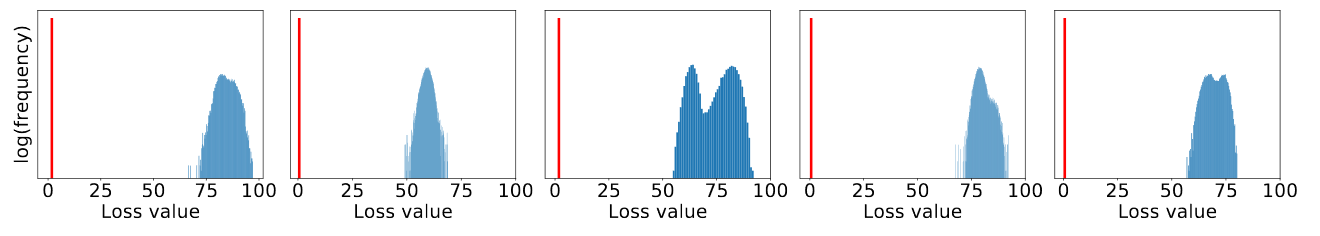
\includegraphics[width=0.99\textwidth,keepaspectratio]{img/other/pgd_histogram.png}
\caption{Frekvencija vrijednosti funkcije gubitka nakon PGD napada. Napad je proveden na $5$ slika iz $10^{5}$ različitih početnih točaka. Crvenom bojom su označene vrijednosti nakon neprijateljskog treniranja uz PGD, a plavom bojom su označene vrijednosti funkcije gubitka na standardno treniranom modelu. Slika preuzeta iz \citep{Madry2017TowardsDL}.}
\label{fig:pgd_histogram}
\end{figure}

Dakle, korištenjem PGD napada pokazano je da za neki $\boldsymbol{x}$ može biti generirano mnogo različitih neprijateljskih primjera, ali će svi ti neprijateljski primjeri povećati funkciju gubitka do približno iste vrijednosti. Autori su trenirali dva modela: jedan za MNIST te jedan za CIFAR-10. Pokazalo se da je kapacitet mreže od presudne važnosti za uspješnost neprijateljskog treniranja. Razlog tome je što je potrebno jako povećati nelinearnost granice između razreda. Ilustracija toga je na slici \ref{fig:pgd_nonlinearity}. 

\begin{figure}[H]
\centering
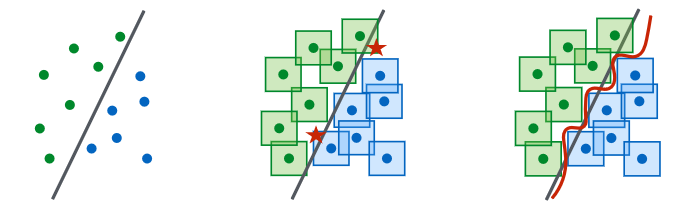
\includegraphics[width=0.99\textwidth,keepaspectratio]{img/other/pgd_nonlinearity.png}
\caption{Na lijevoj slici je pokazana linearna razdvojivost između dva razreda te je granica vrlo jednostavna. Na srednjoj slici su prikazani primjeri uz njihovo $\epsilon$-okruženje. Neprijateljski primjer može biti u okruženju, a pripasti drugom razredu. To je označeno zvjezdicom. Na desnoj slici je nacrtana nelinearna granica koja razdvaja i $\epsilon$-okruženja.} Slika preuzeta iz \citep{Madry2017TowardsDL}.
\label{fig:pgd_nonlinearity}
\end{figure}

Autori su zato koristili široku verziju ResNet mreže koja se razlikuje po većem broju filtera i stoga ima puno veći kapacitet od ``obične'' ResNet mreže. Rezidualne jedinice u ovoj širokoj mreži imaju redom broj filtera: $16$, $160$, $320$, $640$. Na ovoj mreži se može postići točnost od $95.2\%$ na CIFAR-10 uz standardno treniranje. U sklopu ovog rada je testirano PGD neprijateljsko treniranje na standardnoj ResNet-$18$ mreži. Nakon $30$ sati treniranja, postignuta točnost na čistim podatcima je $74.20\%$. Uspješnost neprijateljskih primjera je praktički jednaka kao i na običnom modelu, te nije postignuta veća robusnost modela na neprijateljske primjere. To ukazuje da je veći kapacitet presudan -- standardna ResNet-$18$ mreža ima puno manji kapacitet od dublje široke ResNet mreže i to je najvjerojatniji razlog za neuspjeh ovog pokušaja neprijateljskog treniranja. Za treniranje CIFAR-10 modela opisanog u radu je autorima trebalo $80$ sati. U svrhu evaluacije obrane, autori su organizirali dva ``izazova'' gdje je cilj bio poraziti obranu na MNIST\footnote{\url{https://github.com/MadryLab/mnist_challenge}} i CIFAR-10\footnote{\url{https://github.com/MadryLab/cifar10_challenge}} skupu podataka. 
\\
Za CIFAR-10, najbolji rezultat napada na model crne kutije smanjio je točnost modela na $63.39\%$. Najbolji napad na model bijele kutije smanjio je točnost na $43.99\%$. Iako brojevi možda izgledaju poražavajuće, ovo je i danas jedna od najboljih obrana od neprijateljskih napada. Bitno je podsjetiti se da neprijateljski napadi na druge CIFAR-10 modele i obrane mogu lako spustiti točnost do približno $0\%$.
\\
Za MNIST, najbolji rezultat napada na model crne kutije smanjio je točnost modela na $92.76\%$. Najbolji napad na model bijele kutije smanjio je točnost na $88.06\%$. Ovdje je obrana iznimno uspješna. \\
U trenutku pisanja rada, autori još uvijek prihvaćaju i evaluiraju nove napade na model bijele kutije. Napad koji je spustio točnost CIFAR-10 modela na $43.99\%$ je predan na evaluaciju u veljači $2020.$ godine. Ovo ukazuje na to koliko je područje aktivno i kako problem obrane definitivno nije riješen.
\par
Činilo se da napokon postoji robusna obrana, barem za MNIST skup podataka. Međutim, otvoreni izazov za napad na model crne kutije je bio otvoren samo nekoliko mjeseci u $2017.$ godini. Neko vrijeme nakon toga, autori graničnog napada (opisanog u potpoglavlju \ref{boundary_att}) uspjeli su tim napadom spustiti točnost MNIST modela na $37\%$, a korištenjem napada koji se temelji na $\ell_{0}$ normi su spustili točnost na $0\%$ \citep{towards_mnist}. Ova obrana je ipak pre-trenirana na $\ell_{\infty}$ normu. Postavlja se onda pitanje zašto je najbolji napad na model bijele kutije smanjio točnost samo do $88.06\%$ iako je izazov još uvijek otvoren. Ovo je znak da je i neprijateljsko treniranje oblik maskiranja gradijenata, odnosno da je mreža naučila pri treniranju kako sakriti gradijente i tako spriječiti napade. Napadi na model crne kutije bi, na robusnom modelu, trebali biti slabiji od napada na model bijele kutije. Usprkos tome, ovo je i dalje \textit{state-of-the-art} obrana, ali bitno je naglasiti da je uspješna samo za $\ell_{\infty}$ normu.
\pagebreak
\section{Budući rad}
Obrana od neprijateljskih primjera još uvijek stoji kao neriješen problem. Do sada najuspješnija metoda je neprijateljsko treniranje uz PGD napad, međutim i ta metoda nije u potpunosti robusna: pretrenirana je na $\ell_{\infty}$ normu, slaba je na postojeće napade na model crne kutije i vrijeme treniranja sprječava korištenje obrane na većim skupovima podataka kao što je ImageNet. Budući rad na području obrane se može potencijalno razvijati u nekoliko smjerova. \par
Jedan od smjerova razvoja koji nije razmatran u ovom radu je formalna dokazivost robusnosti modela. Iako postoji mnogo uspješnih radova na tu temu, pristupi nisu primjenjivi na modele korištene u praksi. Često tehnike za dokazivanje robusnosti zahtijevaju da neuronska mreža bude posebno konstruirana kako bi tehnika bila primjenjiva, što onda nije primjenjivo na postojeće modele. Postoje i radovi na temu metoda dokazivanja robusnosti modela u generalnom slučaju, no takve metode su u praksi teško izračunljive čak i za vrlo jednostavne mreže. Dodatna prepreka ovih metoda je što često mogu garantirati robusnost samo za unaprijed određeni skup podataka, a u praksi se želi postići robusnost generalnog oblika. \par
Drugi smjer bi bio daljnji razvoj metoda koje se temelje na neprijateljskom treniranju. Početkom $2020.$ godine je izašao rad upravo na tu temu gdje su autori uspješno neprijateljski trenirali CIFAR-10 i ImageNet mreže u vrlo kratkom roku \citep{fbf}. CIFAR-10 mreža je nakon $6$ minuta postigla robusnu točnost od $45\%$ za $\epsilon = 8 / 255$, a ImageNet mreža je postigla robusnu točnost od $43\%$ za $\epsilon = 2 / 255$ nakon $12$ sati treniranja. Autori su zapravo osmislili način treniranja korištenjem FGSM napada umjesto PGD napada, ali tako da se izbjegne pretreniranost koja je pokazana u poglavlju \ref{adv_fgsm} što je omogućilo puno brže treniranje od iterativnog PGD napada. \par
Treći smjer, što je vjerojatno i najneuspješniji smjer do sada, su nove tehnike obrane bazirane na nekoj heuristici. Takve su na primjer bile termometarsko kodiranje (\ref{thermometer}) i obrambena destilacija (\ref{def_destil}). Obrane bazirane na proizvoljnoj heuristici su se redovito pokazale samo prividno uspješnima. No neuspjeh postojećih metoda ne mora nužno ukazivati na budući neuspjeh sličnih obrana te svaka nova takva obrana do neke mjere produbljuje teorijsko znanje o neprijateljskim primjerima čak i kada se kasnije pokaže da je slaba. Ove metode su potaknule razvoj vrlo jakih napada koji su danas standardni pri evaluaciji obrana (\ref{cw}). \par
U kontekstu ovog rada, opisan je samo mali dio bogatog područja neprijateljskih primjera. Rad je fokusiran na neprijateljske primjere i obrane u području raspoznavanja objekata, no neprijateljski primjeri su općeniti pojam koji se može primijeniti na široki skup domena (npr. raspoznavanje govora i detekcija zloćudnih programa). Također, rad nije ulazio pretjerano duboko u ideju neprijateljskog treniranja što je već sada jako široko područje gdje novi radovi izlaze vrlo često, ponekad i više puta dnevno\footnote{\url{https://nicholas.carlini.com/writing/2019/all-adversarial-example-papers.html}}. Budući diplomski radovi će zasigurno moći evaluirati puno robusnije i uspješnije metode obrane nego ovaj rad jer je istraživanje neprijateljskih primjera vrlo aktivno područje i samo je pitanje vremena kada će se pojaviti još bolja obrana od postojećih. 

\chapter{Zaključak}
Konvolucijske neuronske mreže su se pokazale iznimno uspješnima pri rješavanju problema klasifikacije slika. Međutim, pojava neprijateljskih primjera dovela je u pitanje tvrdnju da današnji modeli dobro generaliziraju. Također se ispostavilo da je vrlo lako osmisliti uspješne algoritme koji mogu generirati neprijateljske primjere, a za neke napade čak nije potrebno nikakvo znanje o mreži koju se napada. Ubrzo nakon pojave neprijateljskih primjera su se pojavile i prve potencijalne obrane. Iako su sve obrane na prvi pogled izgledale obećavajuće, protiv njih su konstruirani napadi koji ih s lakoćom zaobilaze. Od svih obrana do sada, gotovo niti jedna obrana nije znatno povećala robusnost modela. Najviše obećavajuća obrana do sada temelji se na treniranju mreže korištenjem neprijateljskih primjera stvorenih PGD napadom, no uspješnost obrane jako ovisi o kapacitetu modela, a to je ono što tu obranu čini skupom i neuporabljivom na većim skupovima podataka kao što je ImageNet. Obrana od neprijateljskih primjera i dalje stoji kao neriješen problem, a budućnost obrana još uvijek nije očita. Praktički svaki dan se pojavljuju sve djelotvornije i učinkovitije metode temeljene na neprijateljskom treniranju, formalni postupci koji mogu dokazati robusnost mreže te potpuno nove metode obrana koje će tek biti detaljno evaluirane. 


\bibliographystyle{fer}
\bibliography{literatura}

\chapter{Privitak}\label{dodatak}
\section{Osobni skup slika}\label{osobni_skup}
U skupu slika \ref{ref_personal_image_table} je $16$ slika i labela koje su u radu korištene za generiranje suparničkih primjera za modele trenirane na ImageNet skupu podataka. Sve slike su odabrane tako da spadaju unutar $1000$ razreda za koje su modeli predviđeni, dakle slike bi trebale biti ispravno klasificirane. Također, sve slike su unaprijed izrezane u oblik kvadrata kako ne bi došlo do prevelike degradacije kvalitete pri smanjenju rezolucije na $224\times224$. Ovim putem se zahvaljujem Sarah James na dopuštenju za korištenje slika u radu.

\section{Izlazi modela na nepromijenjenim slikama iz osobnog skupa}
Slike iz \ref{osobni_skup} su birane tako da budu reprezentativne za pojedinu klasu, odnosno da ne postoji mogućnost da su mreže ``zbunjene'' oko toga što je na slici. Ideja iza toga je pokazati kako je neprijateljske primjere lako konstruirati čak i kada je mreža iznimno sigurna u to što vidi na slici. U tablici \ref{regular_predictions} nalaze se top-1 izlazi mreža ResNet50V2 (primarna mreža korištena kroz rad) i Xception.
\\
\bgroup
\def\arraystretch{1.2}
\begin{table}[H]
\begin{tabular}{|c | c | c|}
\hline
Slika & ResNet50 V2 & Xception \\ \hline
\ref{ref_pi01} & African grey $100.00\%$ & African grey $100.00\%$  \\ \hline
\ref{ref_pi02} & Backpack $99.71\%$ & Backpack $99.99\%$ \\ \hline
\ref{ref_pi03} & Dragonfly $99.93\%$ & Dragonfly $99.79\%$ \\ \hline
\ref{ref_pi04} & Bald eagle $87.47\%$ & Bald eagle $99.62\%$ \\  \hline
\ref{ref_pi05} & Grocery store $90.81\%$ & Grocery store $97.68\%$ \\ \hline
\ref{ref_pi06} & Gorilla $99.83\%$ & Gorilla $99.96\%$ \\ \hline
\ref{ref_pi07} & Guinea pig $100.00\%$ & Guinea pig $99.99\%$ \\ \hline
\ref{ref_pi08} & Jack-o'-lantern $100.00\%$ & Jack-o'-lantern $99.89\%$ \\ \hline
\ref{ref_pi09} & Jigsaw puzzle $100.00\%$ & Jigsaw puzzle $100.00\%$ \\ \hline
\ref{ref_pi10} & Computer keyboard $65.34\%$ & Computer keyboard $99.68\%$ \\ \hline
\ref{ref_pi11} & Llama $100.00\%$ & Llama $100.00\%$ \\ \hline
\ref{ref_pi12} & Meerkat $99.98\%$ & Meerkat $99.89\%$ \\ \hline
\ref{ref_pi13} & English Springer $88.93\%$ & English Springer $99.30\%$ \\ \hline
\ref{ref_pi14} & Running shoe $80.76\%$ & Running shoe $99.48\%$ \\ \hline
\ref{ref_pi15} & Tabby $64.28\%$ & Tabby $89.72\%$ \\ \hline
\ref{ref_pi16} & Wardrobe $87.16\%$ & Wardrobe $79.05\%$ \\ \hline
\end{tabular}
\caption{Tablica top-1 izlaza mreža ResNet50 V2 i Xception za slike iz \ref{osobni_skup}.}\label{regular_predictions}
\end{table}
\egroup

\begin{figure}[H]
    \centering
    % images 1-4
    \subfloat[\textit{African grey} (87)]{
        \label{ref_pi01}
        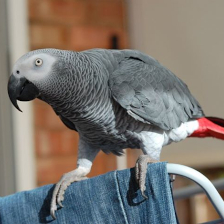
\includegraphics[width=0.25\textwidth]{img/personal_images/african_grey.jpg}
    }
    \subfloat[\textit{Backpack} (414)]{
        \label{ref_pi02}
        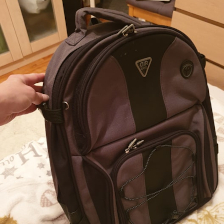
\includegraphics[width=0.25\textwidth]{img/personal_images/backpack.jpg}
    }
    \subfloat[\textit{Dragonfly} (319)]{
        \label{ref_pi03}
        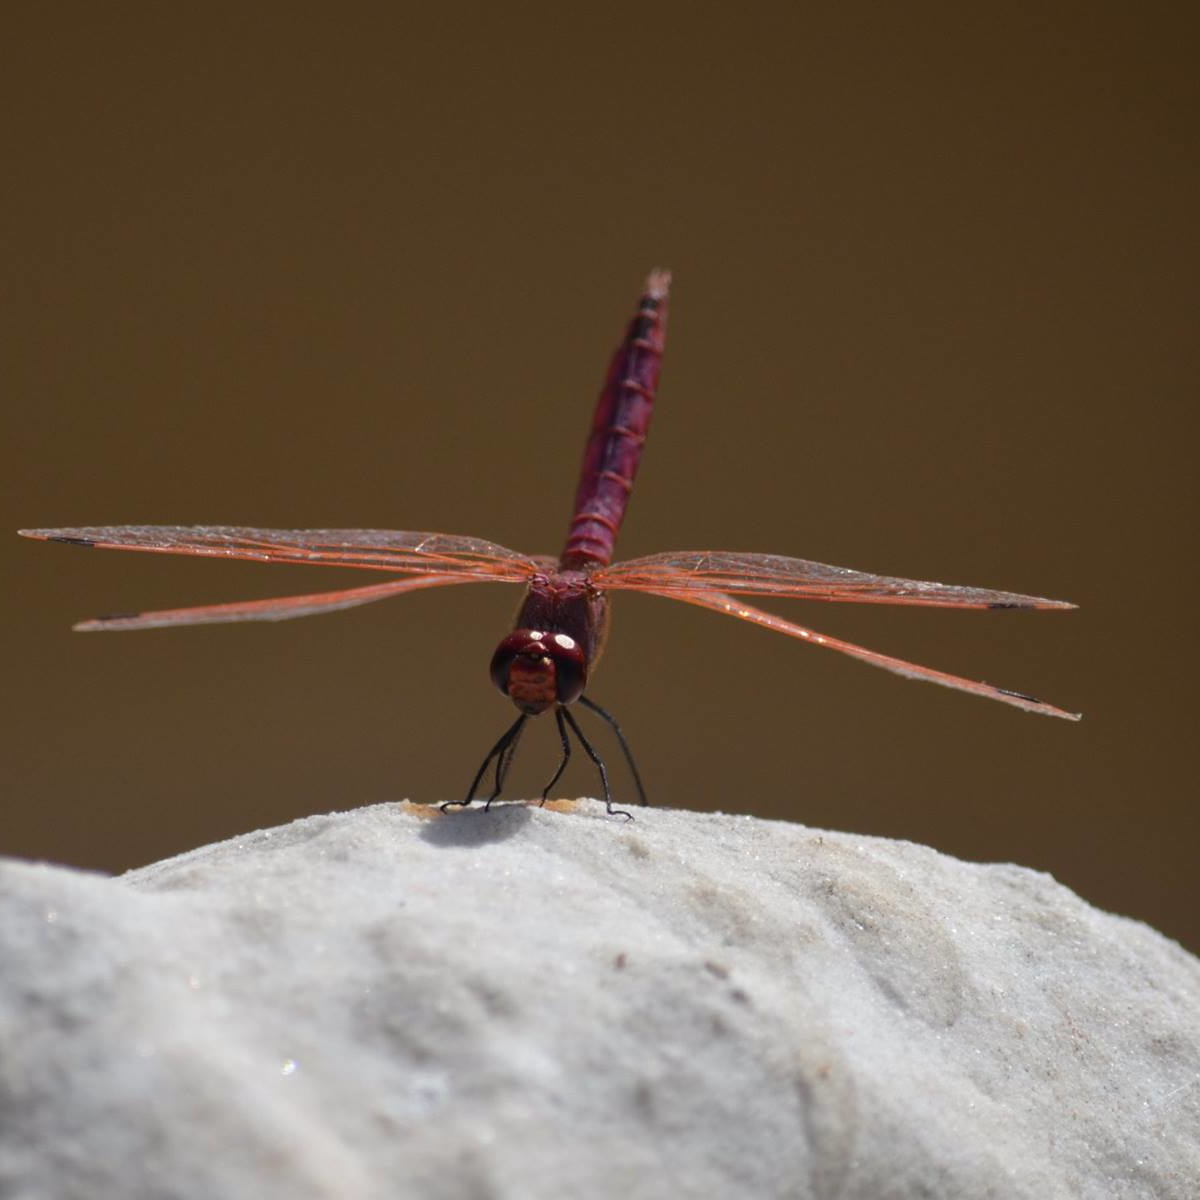
\includegraphics[width=0.25\textwidth]{img/personal_images/dragonfly.jpg}
    }
    \subfloat[\textit{Bald eagle} (22)]{
        \label{ref_pi04}
        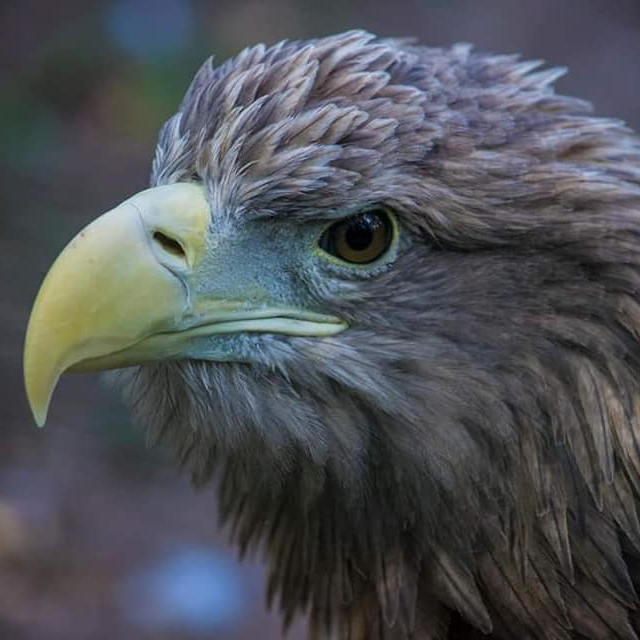
\includegraphics[width=0.25\textwidth]{img/personal_images/eagle.jpg}
    }
    \newline
    % images 5-8
    \subfloat[\textit{Grocery store} (582)]{
        \label{ref_pi05}
        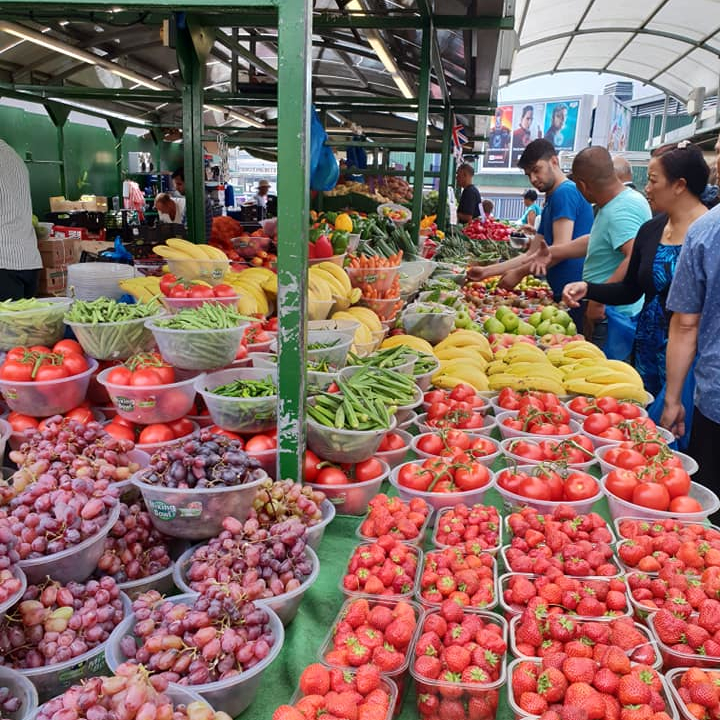
\includegraphics[width=0.25\textwidth]{img/personal_images/food_market.jpg}
    }
    \subfloat[\textit{Gorilla} (366)]{
        \label{ref_pi06}
        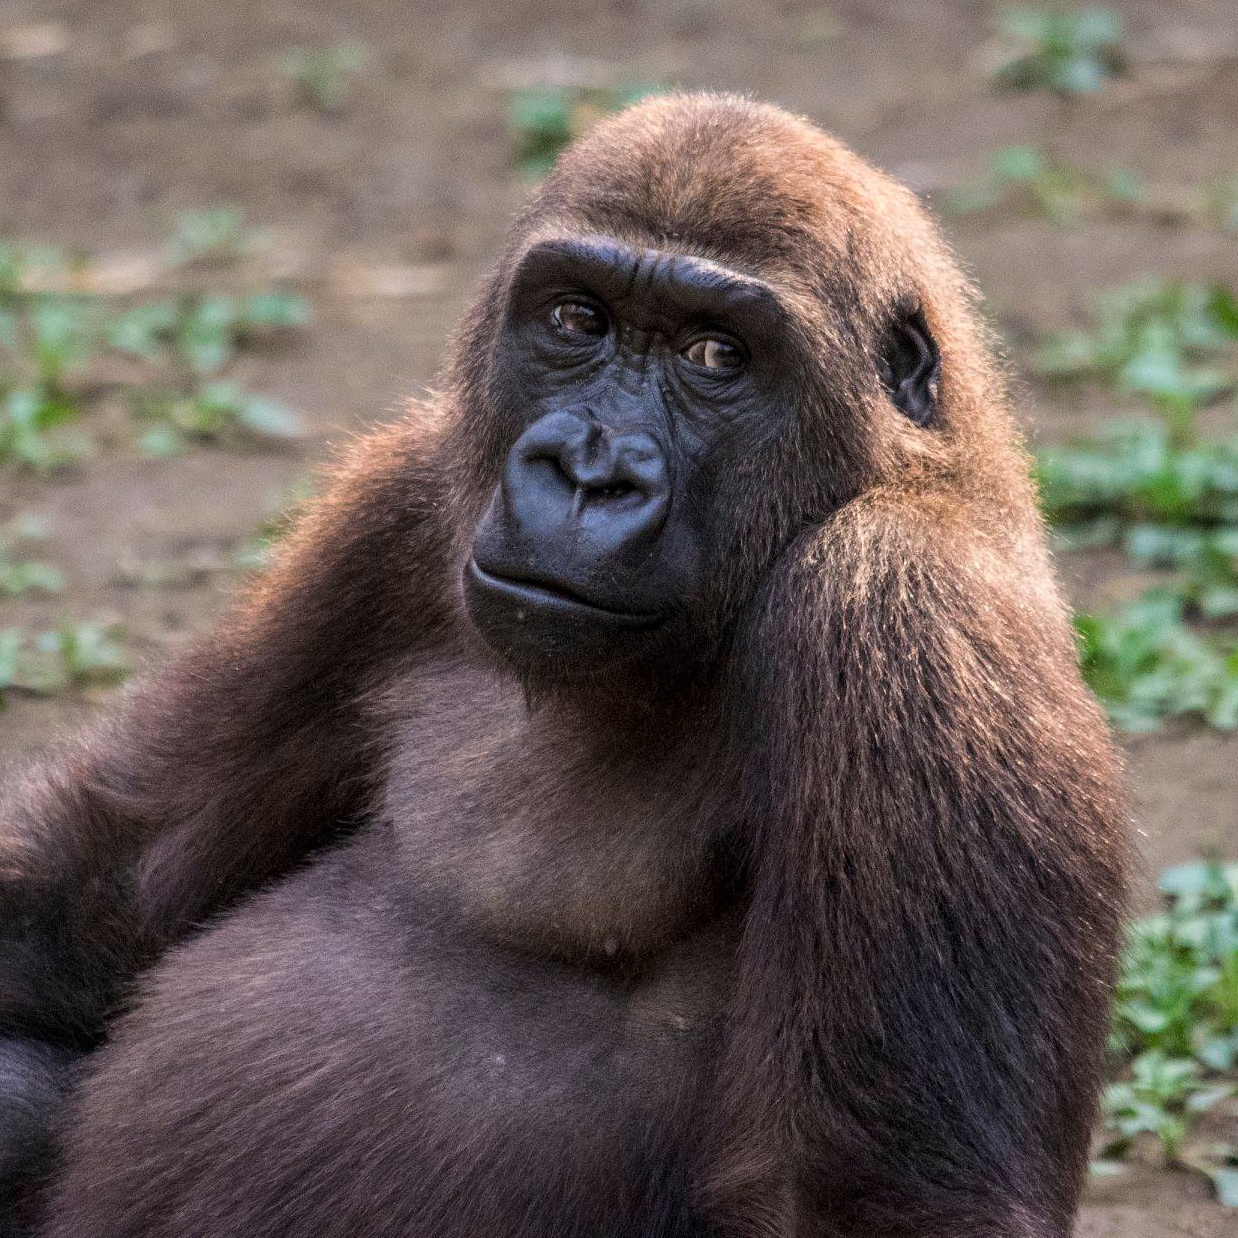
\includegraphics[width=0.25\textwidth]{img/personal_images/gorilla.jpg}
    }
    \subfloat[\textit{Guinea pig} (338)]{
        \label{ref_pi07}
        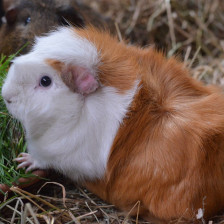
\includegraphics[width=0.25\textwidth]{img/personal_images/guinea_pig.jpg}
    }
    \subfloat[\textit{Jack-o'-lantern} (607)]{
        \label{ref_pi08}
        
\includegraphics[width=0.25\textwidth]{img/personal_images/jackolantern.jpg}
    }
    \newline
    % images 9-12
    \subfloat[\textit{Jigsaw puzzle} (611)]{
        \label{ref_pi09}
        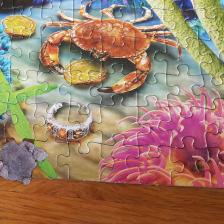
\includegraphics[width=0.25\textwidth]{img/personal_images/jigsaw2.jpg}
    }
    \subfloat[\textit{Keypad} (508)]{
        \label{ref_pi10}
        \includegraphics[width=0.25\textwidth]{img/personal_images/keyboard.jpg}
    }
    \subfloat[\textit{Llama} (355)]{
        \label{ref_pi11}
        \includegraphics[width=0.25\textwidth]{img/personal_images/llama.jpg}
    }
    \subfloat[\textit{Meerkat} (299)]{
        \label{ref_pi12}
        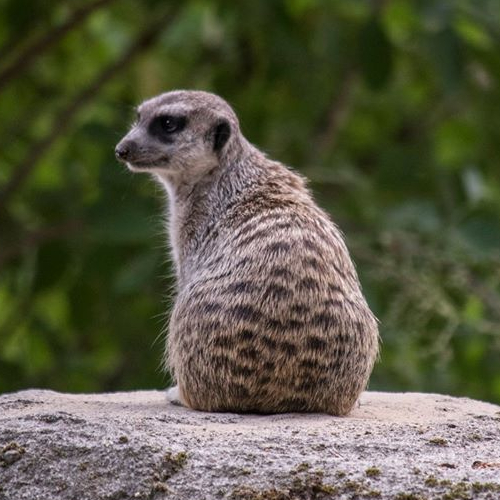
\includegraphics[width=0.25\textwidth]{img/personal_images/meerkat.jpg}
    }
    \newline
    % images 13-16
    \subfloat[\textit{English springer} \newline \centerline{(217)}]{
        \label{ref_pi13}
        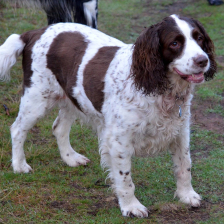
\includegraphics[width=0.25\textwidth]{img/personal_images/megan.jpg}
    }
    \subfloat[\textit{Running shoe} (770)]{
        \label{ref_pi14}
        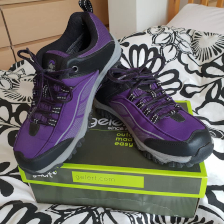
\includegraphics[width=0.25\textwidth]{img/personal_images/running_shoes.jpg}
    }
    \subfloat[\textit{Tabby} (281)]{
        \label{ref_pi15}
        \includegraphics[width=0.25\textwidth]{img/personal_images/tabby.jpg}
    }
    \subfloat[\textit{Wardrobe} (894)]{
        \label{ref_pi16}
        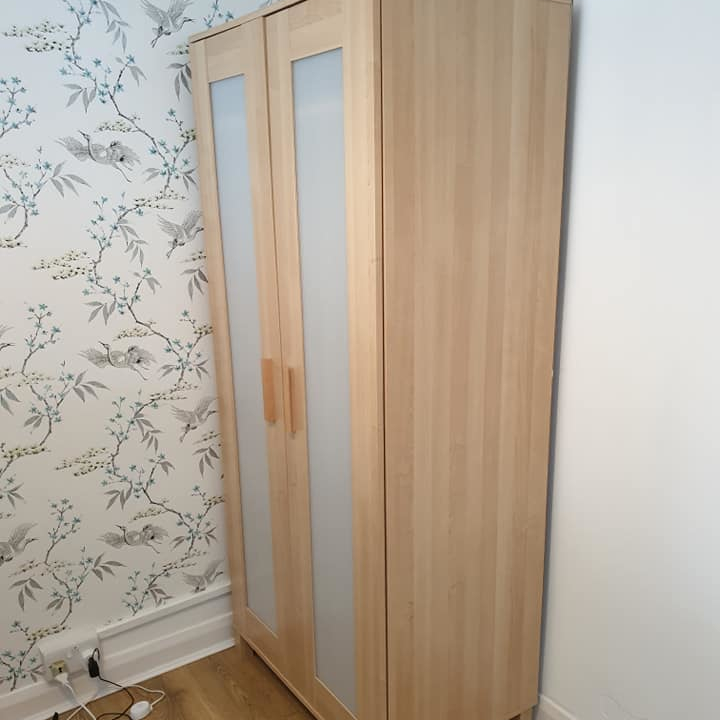
\includegraphics[width=0.25\textwidth]{img/personal_images/wardrobe.jpg}
    }
    
    \caption{Slike korištene za generiranje suparničkih primjera te njihove ispravne labele}
    \label{ref_personal_image_table}
\end{figure}


\begin{sazetak}
Današnji konvolucijski modeli postižu visoku točnost u području raspoznavanja objekata. Način rada dubokih modela je još uvijek vrlo teško ili nemoguće interpretirati, a dodatan razlog za brigu predstavljaju i takozvani neprijateljski primjeri. U kontekstu raspoznavanja objekata, neprijateljski primjeri su slike s dodanim teško uočljivim perturbacijama koje potiču model na pogrešnu klasifikaciju. Pokazalo se da je vrlo lagano konstruirati snažne napade na postojeće modele koji s lakoćom zavaravaju model. Ubrzo nakon pojave prvih neprijateljskih napada su se pojavile i uspješne obrane protiv tih napada, no nedugo nakon toga pojavljuju se sve jači napadi, dok je uspješnost obrana stagnirala. U radu je dan pregled ranijih napada i jednostavnih obrana, istaknuta je neuspješnost jednostavnih obrana protiv jačih napada te je opisana obećavajuća obrana koja se temelji na treniranju mreže korištenjem neprijateljskih primjera.

\kljucnerijeci{klasifikacija objekata, konvolucijske neuronske mreže, računalni vid, suparnički primjeri, neprijateljski primjeri, obrana}
\end{sazetak}
\pagebreak
\engtitle{Defending Deep Convolutional Models from Adversarial Examples}
\begin{abstract}
Today's convolutional models can achieve high accuracy in the field of object recognition. The way deep models work is still very difficult or impossible to interpret, and an additional reason for concern are the so-called adversarial examples. In the context of object recognition, adversarial examples are images with added imperceptible perturbations that encourage the model to misclassify the image. It turned out to be very easy to construct strong attacks on existing models which easily fool the model. Soon after the appearance of the first adversarial attacks, defences against these attacks also appeared. However, stronger attacks appeared not long after that while the success rate of defence methods stagnated. The thesis reviews these early attacks and simple defences and highlights the failure of such defences against strong attackers. Additionally, the thesis describes a promising defence which is based on the concept of adversarial training and has so far shown good results.

\keywords{object classification, convolutional neural networks, computer vision, adversarial attacks, defense}
\end{abstract}
\end{document}
